\chapter{Literature Review}
	\label{chap: literature_review}
	
	\section{Background Information \& Related Work}
		\subsection{Intelligent Transportation Systems (ITS)}
			\subsubsection{What is ITS?}
			Intelligent transport system (ITS) is a general term for the unified applications of communications, control, and information processing technologies to vehicular networks. The subsequent benefits save lives, time, money, energy, and the environment itself. Fundamental attributes of ITS cover all approaches of transport and imitate all features of the transportation system: the vehicle, the infrastructure, and the driver or user, collaborating together dynamically. The universal purpose of ITS is to develop decision making in real time by vehicular network controllers and other users, thereby filtering the operation of the entire transport network. \\
			Data generated by ITS may offer real-time information about current conditions of roads, or information for journey planning, safer, more harmonized, and more “intelligent” decisions on using the networks. ITS adds information and communications technology to transport infrastructures and vehicles in an effort to improve their safety, reliability, efficiency, and quality. ITS encompasses a broad range of wireless and wire line communication-based information and information processing, control algorithm, electronics, and other technologies. When integrated into the transportation system’s infrastructure, and in vehicles themselves, these technologies relieve congestion, improve safety, and enhance productivity. \\
			ITS is the integration of information and communication technologies in the transportation system, which would improve safety, efficiency, and sustainability. Companies and government are working in tandem to address the current transportation challenges in the present fiscally constrained environment. High investments are being made in ITS to develop cost-effective measures that can lessen the traffic strain, congestion, and carbon emissions, while modernizing the present traffic operations, optimizing system performance, and improving access to transportation alternatives. \\
			The navigation and communication technologies that are typically used in ITS are global positioning system (GPS), dedicated short-range communication (DSRC), and carrier access for land mobiles (CALM). The vehicle detection system, traffic information, and variable message signs are the essential elements in an ITS, all of which improve the efficiency and reliability of the transportation infrastructure. ITS uses various systems, namely the Advanced Traffic Management System (ATMS), Advanced Traveler Information System (ATIS), ITS-Enabled Transportation Pricing System, Advanced Public Transportation System (APTS), and Commercial Vehicle Operation (CVO). These systems can be used for various applications like asset monitoring, parking management, collision avoidance systems, traffic monitoring, and traffic enforcement cameras. \\
			ITS can be defined as the application of advanced sensor, computer, electronics, and communication technologies and management strategies in an integrated manner to improve safety and efficiency of the surface transportation system. ITS has the potential to solve the most common challenges related to recent transportation systems, such as heavy traffic congestion in large cities, poor traffic management, unreliable services, and so forth. Moreover, it is shown that ITS has the possibility to act as a key factor for economic growth in many countries \cite{buyya2016internet}. 
			
			\subsubsection{ITS Applications}
			\begin{itemize}
				\let\labelitemi\labelitemii
				\item Travel and transportation management
				\item Travel demand management
				\item Public transportation operation
				\item Electronic payment
				\item Commercial Vehicle Operation (CVO)
				\item Emergency management
				\item Advanced vehicle control and safety system
			\end{itemize}
			
			\subsection{Vehicular Ad-Hoc Network (VANET)}
			\subsubsection{What is VANET?}
			Vehicular ad hoc network (VANET) is a specific case of wireless multi-hop network, which has the constraint of fast topology duo to high node mobility. With the increasing number of vehicles equipped with computing technologies and wireless communication devices, inter-vehicle communication is becoming a hot topic of research, standardization, and development. VANETs enable a wide range of applications, such as prevention of collisions, safety, blind crossing, dynamic routing scheduling, real-time traffic condition monitoring, etc. VANETs also provide Internet connectivity to vehicular nodes \cite{obaidat2015modeling}. An example of a vehicular ad-hoc network is shown in Fig. \ref{fig:vanet1}. 
			\begin{figure}[H]
				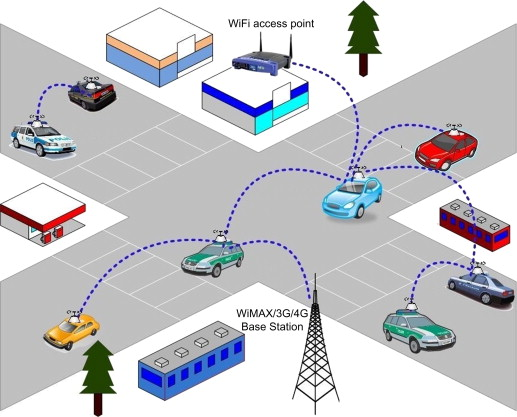
\includegraphics[width=0.65\columnwidth]{{../images/chapter2/vanet1.jpg}}
				\centering
				\caption{An Example of a VANET \cite{obaidat2015modeling}.}
				\label{fig:vanet1}
			\end{figure}
			In VANET, communication between nodes can be classified as vehicle-to-vehicle (V2V), vehicle-to-roadside (V2R), or vehicle-to-infrastructure (V2I). Road-side units (RSUs) are static nodes deployed along the road, which are used to improve connectivity and service provision. RSUs can be connected to a core network and the Internet \cite{rodrigues2020advances}. 
			\begin{figure}[H]
				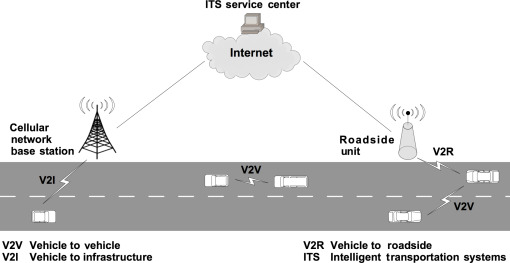
\includegraphics[width=\columnwidth]{{../images/chapter2/vanet3.jpg}}
				\centering
				\caption{Communication Scenarios in VANETs \cite{rodrigues2020advances}.}
				\label{fig:vanet3}
			\end{figure}
			
			\subsubsection{VANET Applications}
			VANET applications are classified in a variety of ways in the literature. The first classification includes four types of applications according to the aim of application: 
			\begin{enumerate}
				\item General information services
				\item Vehicle safety information services
				\item Individual motion control
				\item Group motion control
			\end{enumerate}
			Another classification includes three categories of applications: 
			\begin{enumerate}
				\item Active road safety application
				\item Traffic efficiency and management applications
				\item Infotainment applications
			\end{enumerate}
			\begin{figure}[H]
				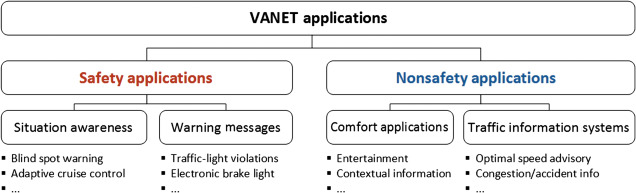
\includegraphics[width=\columnwidth]{{../images/chapter2/vanet4.jpg}}
				\centering
				\caption{Classification of VANET Applications \cite{obaidat2016smart}.}
				\label{fig:vanet4}
			\end{figure}
			Another classification is shown in Fig. \ref{fig:vanet4}. Applications in VANETs are generally classified as safety or non-safety applications. Safety applications include spreading an alarm or warning with the aim of avoiding danger and reducing risks. Non-safety applications include information about a new product or business, the closest restaurant or gas station, or the shortest path to a destination \cite{obaidat2016smart}.
			
			\subsubsection{Security Requirements and Challenges for VANET \cite{paul2016intelligent}}
			VANET is prone to attacks, such as Sybil attack, Denial-of-Service (DoS) attacks, Man-in-the-middle attack, Replay attack, etc. To protect VANET services against these attacks, a set of security primitives should be considered. These security needs are identified at different locations of the architecture based on the characteristics of the transmitted information. 
			\begin{itemize}
				\let\labelitemi\labelitemii
				\item Authentication
				\item Integrity
				\item Non-repudiation
				\item Confidentiality
				\item Access control
				\item Privacy
				\item Accessibility
				\item Responsibility enforcement
				\item Evidence and proof management
				\item Vehicle tracking
			\end{itemize}
			Moreover, mobility constitutes a barrier of the implementation of traditional security schemes in VANETs. Vehicles move at a fast rate, moving in and out of the reception area of other vehicles participating in the network. We can expect that a pair of vehicles can communicate for a limited period of time. It’s also expected that communication between nodes that have interacted before and will never interact again will be the norm. Thus, VANETs are different from existing MANETs where communication between pairs of nodes can be relatively long duration. 
			
			\newpage
			\subsection{Internet of Vehicles (IoV)}
			\subsubsection{What is IoV?}
			The new era of the Internet of Things (IoT) is driving the evolution of conventional vehicular ad-hoc networks (VANETs) into the Internet of Vehicles (IoV). IoV is the type of IoT in the field of transportation (i.e., vehicles). IoV refers to the real-time data intersubsection between vehicles and roads, vehicles and vehicles, as well as vehicles and cities, using mobile-communication technology, vehicle navigation systems, smart-terminal devices, and information platforms to enable information exchange/interaction and a driving-instruction-controlling network system. \\
			IoV enables the gathering and sharing of information regarding vehicles, roads, and their surroundings. IoV is an integrated network for supporting intelligent traffic management, intelligent dynamic information services, and intelligent vehicle control, representing a typical application of IoT technology in intelligent transportation systems (ITS). \\
			IoV is a complex integrated network system, which connects people within vehicles, different vehicles, and different environmental entities of within cities. With the rapid development of computation and communications technologies, IoV promises huge commercial interest and research value. 
			
			\subsubsection{IoV Network Architecture \cite{buyya2016internet}}
			Vehicles in IoV are smart-vehicles with complex intra-vehicle systems. In particular, there are various sensors to collect vehicle and driving status, and communication devices to communicate with other vehicles and/or the Internet. In IoV, vehicles play a dual role: they are clients to consume the service from the Internet and at the same time they are peers to perform distributed computing. IoV is a hybrid system with both peer-to-peer (P2P) and client-server computing paradigms. With a peer-to-peer paradigm, vehicles can cooperate and collaborate with each other to realize distributed-computing functionalities, such as file sharing and cooperative driving. With the client-server paradigm, vehicles can use the resources at servers from the Internet. \\
			IoV consists of two different types of wireless connections. First, Vehicle-to-Vehicle (V2V) communication is used to exchange information among vehicles directly. Wireless links of V2V connect vehicles in an ad-hoc way and construct VANETs. The second type of connections is Vehicle-to-Road (V2R), also called Vehicle-to-Infrastructure (V2I). V2R refers to the information exchange between vehicles, and to road-side infrastructure equipped with wireless communication technology, such as traffic lights or warning signs for roadwork. Unlike V2V, V2R can reach long distances and achieve high scalability. With V2V and V2R communications, IoV can realize information exchange among vehicles, road-side infrastructure, and also the Internet. Then, various applications can be supported by IoV, including ITS and Internet services. IoV network architecture is shown in Fig. \ref{fig:iov1}. 
			\begin{figure}[H]
				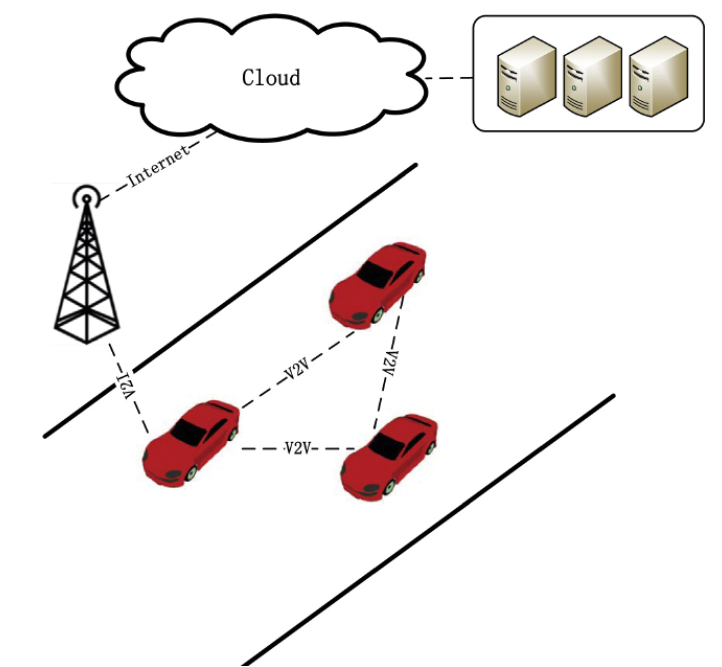
\includegraphics[width=0.42\columnwidth]{{../images/chapter2/iov1.png}}
				\centering
				\caption{IoV Network Architecture \cite{buyya2016internet}.}
				\label{fig:iov1}
			\end{figure}
			
			\subsubsection{IoV Characteristics and Challenges \cite{buyya2016internet}}
			Vehicular networks are mainly composed of vehicle nodes, which behave quite differently from other wireless nodes. Therefore, a vehicular network has several characteristics that may affect the design of IoV technologies. Some characteristics will bring challenges to IoV technological development, whereas some others may bring benefit. Some of IoV characteristics are: 
			\begin{itemize}
				\let\labelitemi\labelitemii
				\item Highly dynamic topology
				\item Variable network density
				\item Large-scale network
				\item Geographical communication
				\item Predictable mobility
				\item Sufficient energy and storage
				\item Various communication environment
			\end{itemize}
			The objective of IoV is to integrate multiple users, multiple vehicles, multiple things, and multiple networks, to always provide the best connected communication capability that is manageable, controllable, operational, and credible. It composes a truly complex system. Moreover, the applications of IoV are quite different from those of other networks, and, consequently, many special requirements arise. Both of these two aspects bring new technical challenges to IoV research and development like: 
			\begin{itemize}
				\let\labelitemi\labelitemii
				\item Poor network connectivity and scalability
				\item Hard delay constraints
				\item High reliability requirements
				\item High scalability requirements
				\item Security and privacy
				\item Service sustainability
			\end{itemize}
			
			\subsubsection{IoV Applications \cite{buyya2016internet}}
			The applications of IoV are quite diverse. According to functionalities, they can be categorized into three major classes. A detailed taxonomy is shown in Fig. \ref{fig:iov2}.
			\begin{figure}[H]
				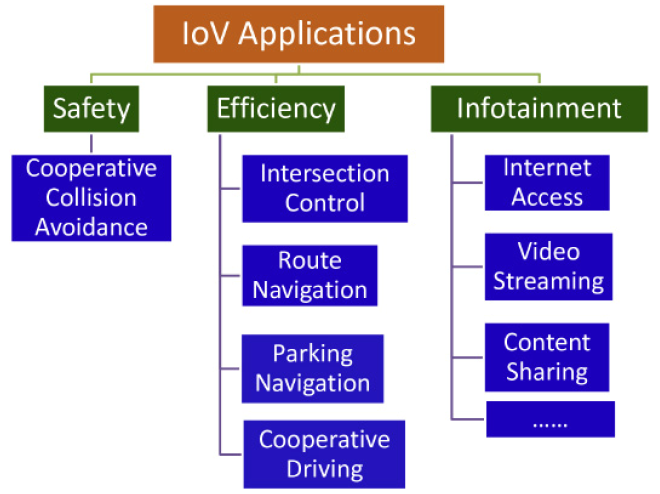
\includegraphics[width=0.53\columnwidth]{{../images/chapter2/iov2.png}}
				\centering
				\caption{A Taxonomy of IoV Applications \cite{buyya2016internet}.}
				\label{fig:iov2}
			\end{figure}
			
			\newpage
			\subsection{Cryptography \cite{paar2009understanding}}
				\subsubsection{Cryptography Terminology}
					\begin{figure}[H]
						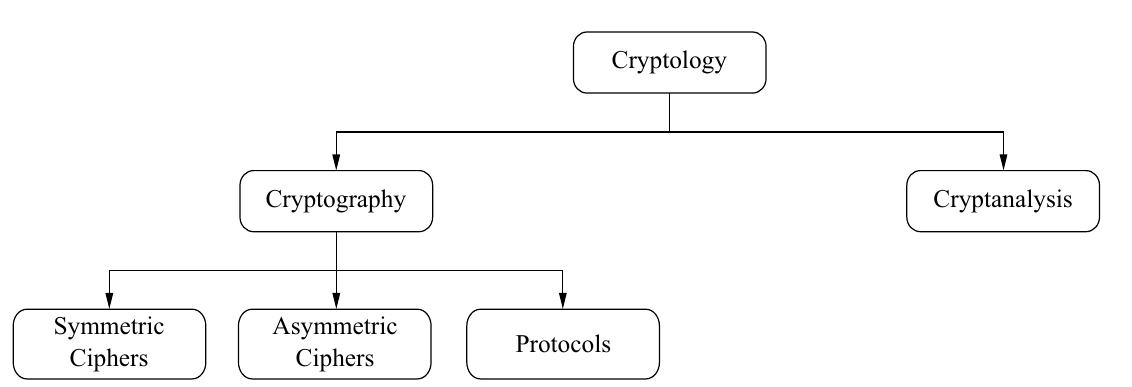
\includegraphics[width=\columnwidth]{{../images/chapter2/crypto1.png}}
						\centering
						\caption{Overview of the field of Cryptology \cite{paar2009understanding}.}
						\label{fig:crypto1}
					\end{figure}
					As shown in Fig.\ref{fig:crypto1}, There are two main branches: 
					\begin{itemize}
						\item \textbf{Cryptography:} the science of secret writing with the goal of hiding the meaning of a message. 
						\begin{enumerate}
							\item \textbf{Symmetric Algorithms:} are what many people assume cryptography is about: two parties have an encryption and decryption method for which they share the same secret key. 
							\item \textbf{Asymmetric (or Public-Key) Algorithms:} it looks like the symmetric one except there is no one shared secret key, each one of parties has two keys public key and private key. Public key is used for encryption, private key is used for decryption.
							\item \textbf{Cryptographic Protocols:} Roughly speaking, crypto protocols deal with the application of cryptographic algorithms. Symmetric and asymmetric algorithms can be viewed as building blocks with which applications such as secure Internet communication can be realized. The Transport Layer Security (TLS) scheme, which is used in every Web browser, is an example of a cryptographic protocol. 
						\end{enumerate}
						\item \textbf{Cryptanalysis:} the science and sometimes art of breaking cryptosystems.
					\end{itemize}
					In the majority of cryptographic applications in practical systems, symmetric and asymmetric algorithms (and often also hash functions) are all used together. This is sometimes referred to as hybrid schemes. The reason for using both families of algorithms is that each has specific strengths and weaknesses. 
				
				\subsubsection{Symmetric Cryptography}
					\begin{figure}[H]
						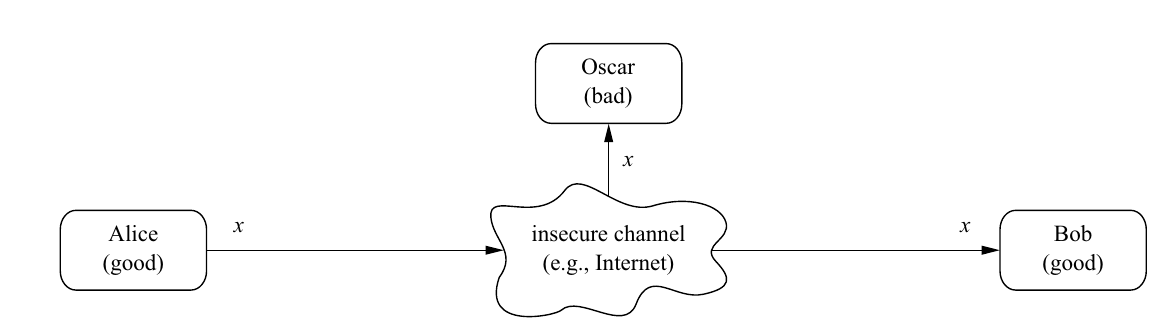
\includegraphics[width=\columnwidth]{{../images/chapter2/crypto2.png}}
						\centering
						\caption{Communication Over an Insecure Channel \cite{paar2009understanding}.}
						\label{fig:crypto2}
					\end{figure}
					There are two users, Alice and Bob, who want to communicate over an insecure channel (Fig. \ref{fig:crypto2}) The actual problem starts with the bad guy, Oscar1 , who has access to the channel, for instance, by hacking into an Internet router or by listening to the radio signals of a Wi-Fi communication. This type of unauthorized listening is called eavesdropping. Obviously, there are many situations in which Alice and Bob would prefer to communicate without Oscar listening. In this situation, symmetric cryptography offers a powerful solution: Alice encrypts her message x using a symmetric algorithm, yielding the ciphertext y. Bob receives the ciphertext and decrypts the message. Decryption is, thus, the inverse process of encryption (Fig. \ref{fig:crypto3}). 
					\begin{figure}[H]
						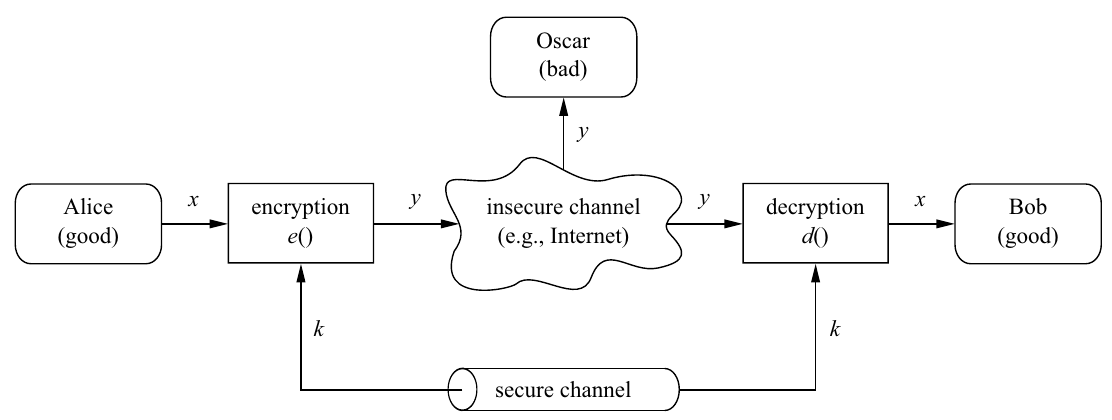
\includegraphics[width=\columnwidth]{{../images/chapter2/crypto3.png}}
						\centering
						\caption{Symmetric-key Cryptosystem \cite{paar2009understanding}.}
						\label{fig:crypto3}
					\end{figure}
					The variables x, y and k in Fig.\ref{fig:crypto3} are important in cryptography and have special names: 
					\begin{itemize}
						\let\labelitemi\labelitemii
						\item \textbf{x} is called plaintext or cleartext,
						\item \textbf{y} is called ciphertext,
						\item \textbf{k} is called the key,
						\item the set of all possible keys is called the key space.
					\end{itemize}
				
				\subsubsection{Asymmetric Cryptography}
					As a system is symmetric with respect to two properties:
					\begin{itemize}
						\let\labelitemi\labelitemii
						\item The same secret key is used for encryption and decryption.
						\item The encryption and decryption function are very similar (in the case of DES they are essentially identical).
					\end{itemize}
					Modern symmetric algorithms such as AES or 3DES are very secure, fast and are in widespread use. However, there are several shortcomings associated with symmetric-key schemes, as discussed below. 
					\begin{itemize}
						\item \textbf{Key Distribution Problem:} The key must be established between Alice and Bob using a secure channel. 
						\item \textbf{Number of Keys:} Even if we solve the key distribution problem, we must potentially deal with a very large number of keys. If each pair of users need a separate pair of keys in a network with n users, there are $\frac{n\cdot\left( n-1\right) }{2}$ key pairs, and every user has to store $\left( n-1\right) $ keys securely. Even for mid-size networks, say, a corporation with $2000$ people, this requires more than $4$ million key pairs that must be generated and transported via secure channels. 
					\end{itemize}
					\paragraph{Principles of Asymmetric Cryptography:}
					\begin{figure}[H]
						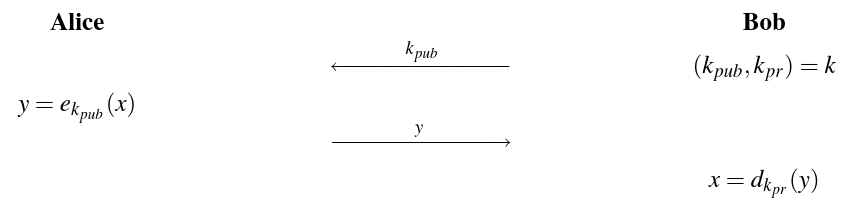
\includegraphics[width=\columnwidth]{{../images/chapter2/crypto4.png}}
						\centering
						\caption{Basic Protocol for Public-key Encryption \cite{paar2009understanding}.}
						\label{fig:crypto4}
					\end{figure}
					As shown in Fig. \ref{fig:crypto4}, in order to overcome these drawbacks, Diffie, Hellman and Merkle had a revolutionary proposal based on the following idea: It is not necessary that the key possessed by the person 
					who encrypts the message (Alice in our example) is secret. The crucial part is that Bob(the receiver) can only decrypt using a secret key. In order to realize such a system, Bob publishes 
					a public encryption key which is known to everyone. Bob also has a matching secret key, which is used for decryption. Thus, Bob's key S consists of two parts, a public part $K_{pub}$ and a private one $K_{pr}$. 
				
				\subsubsection{Hybrid Cryptography}
					As mentioned, that hybrid schemes is used to take advantages of strengths of each cryptosystem. One of the advantages of symmetric cryptosystem is the speed. Symmetric cryptosystem is faster than asymmetric as it use fixed-width bitwise operations unlike asymmetric cryptosystem, it use mathematical operations like mod and power in addition to finding large prime number that cannot be factorized. But asymmetric cryptosystems have a powerful property as there are pair of keys for encryption and decryption. \\
					As shown in Fig. \ref{fig:crypto5} Alice sends his public key($K_{pub}$) to Bob. Then, Bob Generates a session key $K_S$ and encrypts it with alice's public key. Then, Alice decrypt the session key with his private key $K_{pr}$ to obtain the session key.
					At this point the Asymmetric cryptography is done and now the turn of symmetric cryptography.
					Alice can encrypt the message by the session key $K_s$ using any symmetric cryptography algorithm i.e. AES, DES or 3DES, and send the encrypted message to Bob, then Bob decrypts it to get the message.
					\begin{figure}[H]
						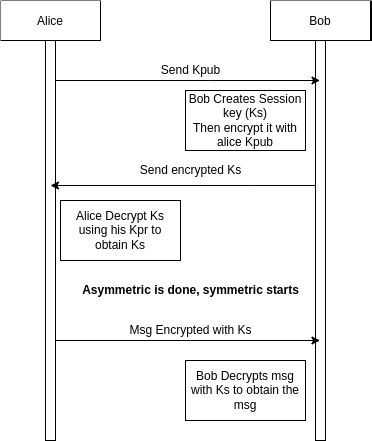
\includegraphics[width=0.55\columnwidth]{{../images/chapter2/crypto5.png}}
						\centering
						\caption{Hybrid Cryptography Algorithm \cite{paar2009understanding}.}
						\label{fig:crypto5}
					\end{figure} 
					
				\subsubsection{Hashing}
					Hash functions are an important cryptographic primitive and are widely used in protocols. They compute a digest of a message which is a short, fixed-length bit-string. For a particular message, the message digest, or hash value, can be seen as the fingerprint of a message, i.e., a unique representation of a message. Unlike all other crypto algorithms , hash functions do not have a key. Hash functions is used to ensure data integrity and secure it against unauthorized modifications. There are a lot of families in hashing functions, like Secure Hash Algorithm SHA, this family of hashes contains SHA-1, SHA-2 and SHA-3, etc. And Message Digest MD, like MD2, MD4 and MD5, etc.
			
			\newpage
			\subsection{Blockchain}
				\subsubsection{What is Blockchain?}
				Blockchain is a distributed public database of all digital events that have been accomplished and shared among participating nodes. It contains a record of every single event ever occurred. Each event in the blockchain database is validated by the consensus of the majority of the nodes in the network. 
				
				\subsubsection{Blockchain Features \cite{shrestha2020new}}
				\begin{itemize}
					\item \textbf{Immutability:} Once a piece of information is recorded, it cannot be modified or deleted from the network, in addition, no arbitrarily or false information can be added.
					\item \textbf{Distributed and the environment is trustless:} Any node can be added can synchronize and validate all content of the blockchain in a decentralized manner which provide security and prevents single point of failure.
					\item \textbf{Privacy and anonymity:} The information about the user cannot be known by the other users and a user can join the network anonymously which means that the personal information is private, anonymous, and secure.
					\item \textbf{Reliable and accurate:} The data in the blockchain are timely and widely accessible, accurate, consistent, and reliable because of the distributed network which means it can withstand malicious attacks and prevent single point of failure problems.
					\item \textbf{Transparency:} Any node in the network can view transactions and the blockchain stores every single transaction in the network which mean complete transparency.
				\end{itemize}
				
				\subsubsection{Blockchain Structure \cite{shrestha2020new}}
				Simply we can refer to the records of the blockchain as “Ledger”, in a simpler term a “List of Blocks”. The root of the ledger (list) is called a genesis block that acts as the first block in the blockchain, and it contains information that is known to all nodes. Blockchain structure is shown in Fig. \ref{fig:blockchain1}. The block has 2 parts Head, and Body: 
				\begin{itemize}
					\let\labelitemi\labelitemii
					\item \textbf{The block header:} Contains of hash of previous block, hash of the current block, nonce, timestamp, and Merkle root. See Fig. \ref{fig:blockchain2}
					\item \textbf{Timestamp:} Is the time in which the block was created.
					\item \textbf{Nonce:} is a number which is used for the hashing problem for mining the block.
					\item \textbf{Merkle root:} is a hashing tree which contains the hashes of the content of the body hashed  recursively so the final hashing is unique for the data contained in the body. 
					\item \textbf{The block body:} contains records of transactions and some other data depending on the functionality of the blockchain. See Fig. \ref{fig:blockchain3} 
					\item \textbf{Transactions:} is the information that is being stored in the block body. \\
					The Idea behind the mentioned structure is that the youngest block added to the ledger is uniquely identified, and very representative to the blockchain so all nodes can easily identify false blocks or false ledgers. 
				\end{itemize}
				\begin{figure}[H]
					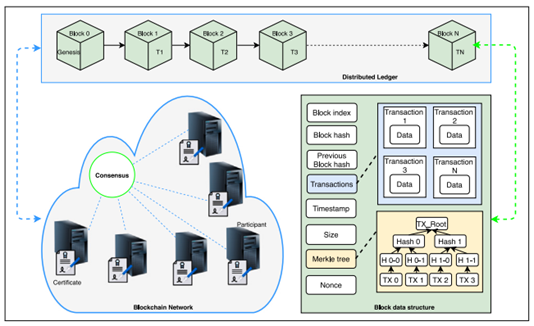
\includegraphics[width=\columnwidth]{{../images/chapter2/blockchain1.png}}
					\centering
					\caption{Blockchain Structure \cite{paper11}.}
					\label{fig:blockchain1}
				\end{figure}
				\paragraph{How the nonce is calculated?} 
				Suppose that the hashing of a block using SHA256 hashing algorithms is: \\ $5fd2f727854b50bb95c054b39c1fe5c92e5ebcfa4bcb5dc279f56aa96a365e5a$\\
				Then if we want to make the first 4 digits to be zero so the hashing would be: \\ $0000f727854b50bb95c054b39c1fe5c92e5ebcfa4bcb5dc279f56aa96a365e5a$\\
				The nonce should be equal to $72608$ to give this hashing. \\
				\textbf{How nonce is calculated?} \textminus It’s calculated by trying the numbers from $1$ to $72608$ trying each value for the specific hashing. For making the problem harder you can give higher constraints like making the $6$ first digits be zero. 
				\begin{figure}[H]
					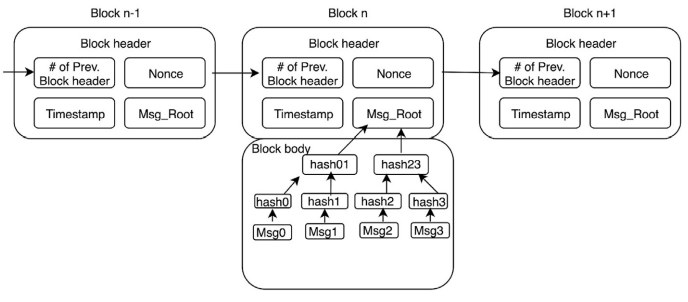
\includegraphics[width=\columnwidth]{{../images/chapter2/blockchain2.png}}
					\centering
					\caption{Sample Chain \cite{shrestha2020new}.}
					\label{fig:blockchain2}
				\end{figure}
				For the older blocks, as the size of the ledger increase it becomes computationally harder for the block to be timbered with, as the hashing problem would require insanely time, power, and computation and hypothetically if the problem was solved the other nodes can easily identify that the ledger is timbered, so the timbering is useless and is not even worth trying. 
				\begin{figure}[H]
					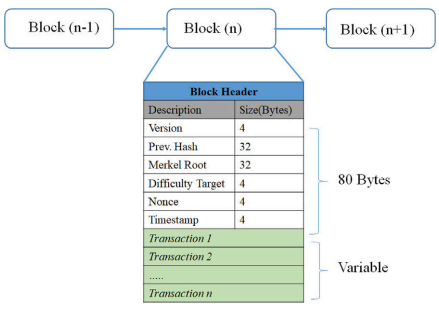
\includegraphics[width=0.7\columnwidth]{{../images/chapter2/blockchain3.png}}
					\centering
					\caption{Single Block Content \cite{shrestha2020new}.}
					\label{fig:blockchain3}
				\end{figure}
				
				\subsubsection{Blockchain Types \cite{blockchain_types}}
				As shown in Fig. \ref{fig:blockchain4}, there are 2 main categories of blockchain, \textbf{permissioned}, and \textbf{permissionless} blockchains.
				\begin{figure}[H]
					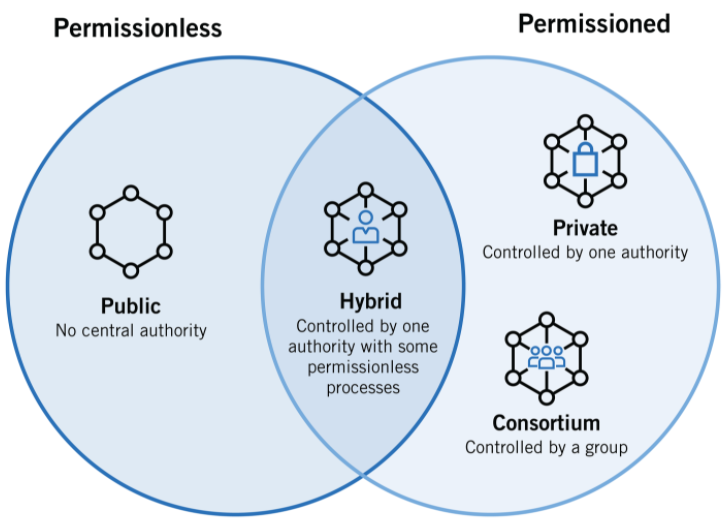
\includegraphics[width=0.63\columnwidth]{{../images/chapter2/blockchain4.png}}
					\centering
					\caption{Blockchain Types \cite{blockchain_types}.}
					\label{fig:blockchain4}
				\end{figure}
			\newpage
				\begin{itemize}
					\item \textbf{Permissionless Blockchains:} \\
					Permissionless blockchains allow any user to pseudo-anonymously join the blockchain network and do not restrict the rights of the nodes on the blockchain network. Permissionless blockchains tend to be more secure than permissioned blockchains because there are numerous nodes to validate transactions, and it would be hard for bad actors to collude on the network. However, permissionless blockchains also tend to have long transaction processing times due to the large number of nodes and the large size of the transactions. 
					\item \textbf{Permissioned Blockchain:} \\
					Permissioned blockchains restrict access to certain nodes to the network and may also restrict the rights of those nodes on that network. The identities of the users of a permissioned blockchain are known to the other users of that permissioned blockchain. Permissioned blockchains tend to be more effective. Because access to the network is restricted, there are lesser nodes on the blockchain, resulting in lower processing time per transaction. \\
					Although the processing time is reduced in permissioned blockchains, the centralization of permissioned blockchains to some central authority (that may be a government, a company, a trade group, or some other entity or group that's granting the authorization to nodes and creating the restrictions of the blockchain) makes it a less secure system that's further prone to traditional hacking vulnerabilities. The fewer nodes there are on a blockchain, the easier it's for bad actors to collude, so private blockchain administrators must ensure nodes adding and verifying blocks are greatly trusted. 
				\end{itemize}
				\textbf{Under the mentioned categories of blockchain there is a number of types which are public, private (managed), consortium, and hybrid blockchains.}
				\begin{itemize}
					\let\labelitemi\labelitemii
					\item \textbf{Public Blockchains:} \\
					Public blockchains are permissionless in nature, allow anyone to join, and are fully decentralized. Public blockchains allow all nodes of the blockchain to have equal rights to access the blockchain, generate new blocks of data, and validate blocks of data. \\
					To date, public blockchains are primarily used for trading and mining cryptocurrency. There are popular public blockchains such as Bitcoin, Ethereum, and Litecoin. On these public blockchains, the nodes “ mine” for cryptocurrency by creating blocks for the transactions requested on the network by solving cryptographic equations. In return for this hard work, the miner nodes earn a small quantity of cryptocurrency. The miners basically act as new era bank tellers that formulate a transaction and take (or “ mine”) a fee for their efforts. 
					\item \textbf{Private Blockchains:} \\
					Private blockchains, which may also be referred to as managed blockchains, are permissioned blockchains controlled by a single organization. In a private blockchain, the central authority determines who can be a node. The central authority also doesn't necessarily grant each node with equal rights to perform functions. Private blockchains are only partly decentralized because public access to these blockchains is limited. Some representatives of private blockchains are the business-to- business virtual currency exchange network Ripple and Hyperledger, an umbrella project of open- source blockchain applications. \\
					Both private and public blockchains have downsides. Public blockchains tend to have longer validation times for new data than private blockchains. Private blockchains are more vulnerable to fraud and bad actors. To address these downsides, consortium, and hybrid blockchains were developed. 
					\item \textbf{Consortium Blockchains:} \\
					Consortium blockchains are permissioned blockchains governed by a group of organizations, rather than one entity, as in the case of the private blockchain. Consortium blockchains, thus, enjoy additional decentralization than private blockchains, influencing in advanced degrees of security. Even so, setting up consortiums can be a fraught process as it requires cooperation between a number of organizations, which presents logistical challenges as well as possible antitrust threat (which we will examine in an forthcoming composition). Further, some members of supply chains may not have the demanded technology nor the infrastructure to implement blockchain tools, and those that do may decide the direct costs are too steep a price to pay to digitize their data and connect to other members of the supply chain. 
					\item \textbf{Hybrid blockchains:} \\
					Hybrid blockchains are blockchains that are controlled by a single organization, but with a degree of oversight performed by the public blockchain, which is needed to perform certain transaction validations. A case of a hybrid blockchain is IBM Food Trust, which was developed to improve efficiency throughout the whole food supply chain. 
				\end{itemize}
				
				\subsubsection{Consensus Algorithms \cite{shrestha2020new}}
				In the blockchain, a consensus is a fault-tolerant mechanism, which is used to accomplish necessary agreement on a single state of the network in a distributed multi-node system. It is a set of rules that decide on the contributions of different participating nodes of the blockchain. 
				\begin{itemize}
					\item \textbf{Proof of Work (PoW):} \\
					In Proof of Work (PoW) a miner is presented with a difficult mathematical problem, which he needs to solve in order to mine the block. Bitcoin uses proof of work as its consensus algorithm for mining blocks. The miner should possess enough computation power to mine the block, this algorithm is biased to the miner with more computational resources. The miner would find a pool of pending transactions and compete with other miners to find a solution to the mathematical problem, and the miner who first solves the problem will get the rewards. PoW is very easy for others to verify but difficult to produce. 
					\item \textbf{Proof of Stack (PoS):} \\
					Proof of Stake (PoS) is yet another blockchain consensus algorithm which is remarkably different in the way it works. PoS is used by many blockchains in production and very soon Ethereum will release Casper, it’s very own version of PoS. In order to be chosen as the next block creator in PoS, miners/validators are required to stake their tokens/balance. Therefore, the miner has the maximum chance of getting selected as a leader and creating the next block if it has the most amount of currency. If a miner is caught cheating or tampering, it loses its entire stake. Hence, such a restriction makes the miners to be trustworthy. 
					\item \textbf{Practical Byzantine Fault Tolerance (pBFT):} \\
					Practical Byzantine Fault Tolerance consensus algorithm designed to work efficiently in asynchronous systems. A PBFT follows a property that the total number of malicious nodes must not be greater than or equal to one-third of all the nodes in the system. With increasing in the number of nodes, the system becomes more secure. This consensus algorithm is not biased to computation power, but here all the peers get equal amounts of authority, to either add or reject the block. It contain two phases: Request phase and the response phase. In the request phase, an Async Http request is sent to all the participating peers. The participating peers should verify the block and send the response to the peer who has proposed the block, after receiving all the response, if there are at least $⅓$ of peers approve to add the block, the block gets added to the chain, else the transaction would be rejected. 
					\item \textbf{Proof of Activity (PoA):} \\
					PoA is a combination of the two most popular consensus algorithms namely, Proof of Work and Proof of Stake. First, it works according to PoW, where a miner needs to solve a complex cryptographic puzzle. Then, it switches to PoS. The blocks that are mined does not contain any transaction information. These are simply the templates with basic header information and the address of the miner to be rewarded. This header information is then used to select a random group of validators who can sign the block and add it to the blockchain. The more the stake the validator has, the more chances are there to get selected as a validator to sign the block. The fees are divided into the miner and the validators. 
				\end{itemize}
				
				\subsubsection{Advantages and Disadvantages of consensus Algorithms \cite{shrestha2020new}}
				\begin{table}[H]
					\centering
					%\label{}
					\caption{Comparison Between Consensus Algorithms.}
					\begin{tabular}{| m{2cm} | m{7cm} | m{7cm} |}
						\hline
						\begin{center}
							Algorithms
						\end{center} & \begin{center}
							Advantages
						\end{center} & \begin{center}
							Disadvantages
						\end{center} \\
						\hline
						\begin{center}
							PoW
						\end{center} & 
						\begin{mylist}
							\item[\textminus] Completely decentralized. 
							\item[\textminus] Nodes can enter and leave any time.
							\item[\textminus] Easy to implement. 
							\item[\textminus] System destruction cost is huge.	
						\end{mylist} & 
						\begin{mylist}
							\item[\textminus] Energy consumption: Excessive computational power is required for miners therefore it is costly and energy intensive. 
							\item[\textminus] Vulnerability: it is prone to a “51\% attack”.
						\end{mylist} \\
						\hline
						\begin{center}
							PBFT
						\end{center} & 
						\begin{mylist}
							\item[\textminus] Has the ability to provide transaction finality without confirmations. 
							\item[\textminus] All honest nodes are agreeing on the same state of the system at that specific time as a result of their communication with each other. 
							\item[\textminus] Utilizes very less energy compared to PoW.
						\end{mylist} & 
						\begin{mylist}
							\item[\textminus] Only works well with limited consensus group sizes.
							\item[\textminus] Susceptible to “Sybil attacks”.
						\end{mylist} \\
						\hline
						\begin{center}
							PoS
						\end{center} & 
						\begin{mylist}
							\item[\textminus] Does not consume huge amounts of electricity to secure the Blockchain. 
							\item[\textminus] No need for powerful hardware or optimal software.
							\item[\textminus] Much less complicated electrical installation.
						\end{mylist} & 
						\begin{mylist}
							\item[\textminus] Vulnerability: The system can be destroyed if someone with sufficient money is willing to invest in the destruction of the entire system.
						\end{mylist} \\
						\hline
						\begin{center}
							PoA
						\end{center} & 
						\begin{mylist}
							\item[\textminus] Requires less amount of computational power compared to PoW. 
							\item[\textminus] Reduced complexity.
						\end{mylist} & 
						\begin{mylist}
							\item[\textminus] Prone to 51\% attack.
						\end{mylist} \\
						\hline
					\end{tabular}
				\end{table}
				\newpage
				
				\subsubsection{Generations of Blockchain \cite{efanov2018all}}
					As shown in Fig. \ref{fig:blockchain5}, blockchain has three generations: 
					\begin{figure}[H]
						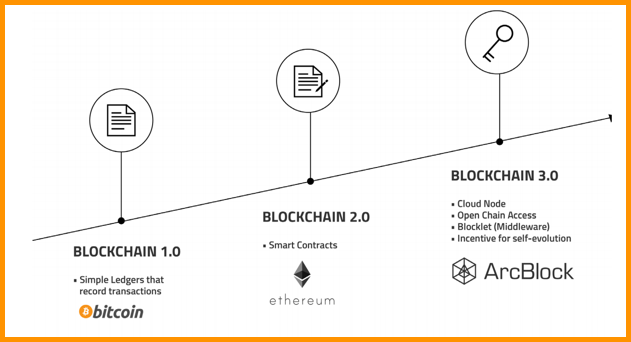
\includegraphics[width=0.7\columnwidth]{{../images/chapter2/blockchain5.png}}
						\centering
						\caption{Blockchain Generations \cite{blockchain_gen}.}
						\label{fig:blockchain5}
					\end{figure}
					\begin{itemize}
						\let\labelitemi\labelitemii
						\item \textbf{Blockchain 1.0 – Digital Currency:} \\
						Blockchain 1.0 is the first generation of blockchain technology applications. It started at 2009 by the introduction of Bitcoin network. The first cryptocurrencies were introduced in this generation. The idea was about generating cryptocurrency and payment and its functionalities. 
						\item \textbf{Blockchain 2.0 – Digital Economy:} \\
						Blockchain 2.0 is the second generation of blockchain it refers to the wide range of economic and financial applications that exist beyond simple payments, transfers, and transactions. \\
						A key emerging use case of the blockchain technology involves smart contracts which are basically computer programs that can automatically execute the terms of a contract. The parties involved in a contractual agreement can be automatically made payments when a pre-configured conditions in a smart contract among participating entities is met. One of the most well-known platforms that runs smart contracts is Ethereum. 
						\item \textbf{Blockchain 3.0 – Digital Society:} \\
						Blockchain 3.0 is the third generation it refers to vast array of applications that do not involve money, currency, commerce, and financial markets. Various research areas like health, governance, IoT, supply-chain, smart city, business, and smart economy. The main features are wider functionality and better scalability. One of the known platforms is ArcBlock. 
					\end{itemize}
			
			\newpage
			\subsection{Cloud Computing}
			\subsubsection{What is Cloud?}
			The cloud" refers to servers which are accessed over the internet, and the software programs and databases that run on those  servers. Cloud servers are placed in data centers all over the world. by way of the use of cloud computing, customers and companies do not have to manipulate physical servers themselves or run software applications on their own machines \cite{cloudref1}. 
			Users can access the same files and applications from almost any device through the cloud because the  computing and storage occur on servers in a data center, instead of local devices of the users. Due to that a user can logs in to its Facebook account on a new phone after the olde one is damaged and still finds his old account as it was in previous containing all his photos, videos, and conversation history. \\
			Switching to cloud computing gits rid of some IT costs and overhead for businesses. for example, businesses no longer need to update and maintain their own servers because the cloud vendor, with who they are subscribed, will do that. Small businesses that may not have been able to afford their own internal infrastructure can now deploy their infrastructure on the cloud with low cost. Another benefit of the cloud for companies is that it makes it easier for them to operate internationally, because employees and customers can access the same files and applications from any location. 
			
			\subsubsection{How Does Cloud Computing Work?}
			Cloud computing depends on a technology called virtualization. Virtualization allows for the creation of a simulated, digital-only "virtual" computer that behaves as if it were a physical computer with its own hardware and is called virtual machine. When Virtualization is properly implemented, virtual machines on the same host machine, which is the physical computer, do not interact with each other at all, and all files and applications from one virtual machine are not visible to the other virtual machines even though they are on the same physical machine. \\
			The concept of virtualization achieves the best making good use of the full hardware resources of a server and this happens when we run many virtual machines at the same time in a way that makes the server becomes many servers simultaneously and a data center becomes a whole host for different data centers where each one of the can serve many organizations. Therefore, cloud providers can offer the use of their servers to far many customers simultaneously, and this can be achieved in low cost. \\
			Cloud servers should be always online and always available which is different from the individual server that sometimes go down. Multiple machines across multiple regions are generally used to back up the different services of the Cloud vendors to achieve reliability and prevent single point of failure. Cloud services can be accessed through a browser or an app which is connected to the internet. 
			
			\subsubsection{Common Service Models of Cloud Computing \cite{cloudref2}}
				As shown in Fig. \ref{fig:cloud2}, cloud services include: 
				\begin{figure}[H]
					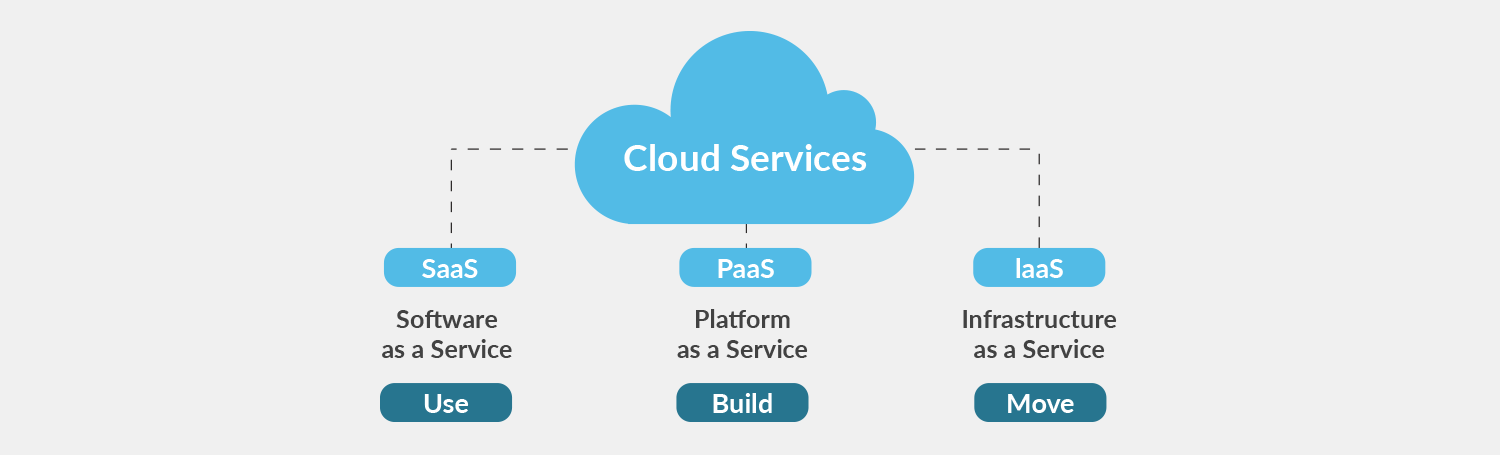
\includegraphics[width=0.9\columnwidth]{{../images/chapter2/cloud2.png}}
					\centering
					\caption{Cloud Services}
					\label{fig:cloud2}
				\end{figure}
				\begin{itemize}
					\item \textbf{Software-as-a-Service (SaaS):} applications are hosted on cloud server instead of users installing them on their local devices and they are accessed over the internet. Some instances for SaaS are Google Workspace, Dropbox, Salesforce, Cisco WebEx, Concur and GoToMeeting. 
					\item \textbf{Platform-as-a-Service (PaaS):} Instead of companies paying for hosted applications, they pay for the things they need to build their own applications. PaaS vendors offer everything necessary for building an application, including development tools, infrastructure, and operating systems, over the Internet. Some PaaS instances are AWS Elastic Beanstalk, Windows Azure, Heroku, Force.com, Google App Engine, Apache Stratos, OpenShift. 
					\item \textbf{Infrastructure-as-a-Service (IaaS):} Renting hardware resources such as servers and storage by companies from a cloud provider such that they then use that cloud infrastructure to build their applications. Some IaaS instances are DigitalOcean, Linode, Rackspace, Amazon Web Services (AWS), Cisco Metapod, Microsoft Azure and Google Compute Engine (GCE). 
				\end{itemize}
			
			\subsubsection{Common Cloud Deployment Types}
				Different cloud types are shown in Fig. \ref{fig:cloud3}: 
				\begin{itemize}
					\item \textbf{Private Cloud:} it is a server, data center, or distributed network wholly dedicated to one organization.
					\item \textbf{Public Cloud:} it is a service run by an external vendor that may include servers in one or multiple data centers. Unlike a private cloud, public clouds are shared by multiple organizations. Using virtual machines, individual servers may be shared by different companies.
					\item \textbf{Hybrid Cloud:} hybrid cloud deployments combine public and private clouds and may even include on-premises legacy servers. An organization may use their private cloud for some services and their public cloud for others, or they may use the public cloud as backup for their private cloud.
					\item \textbf{Community Cloud:} it is built to meet the needs of a specific industry, such as healthcare or media and it is like a public cloud environment, but with set levels of security, and privacy.
				\end{itemize}
				\begin{figure}[H]
					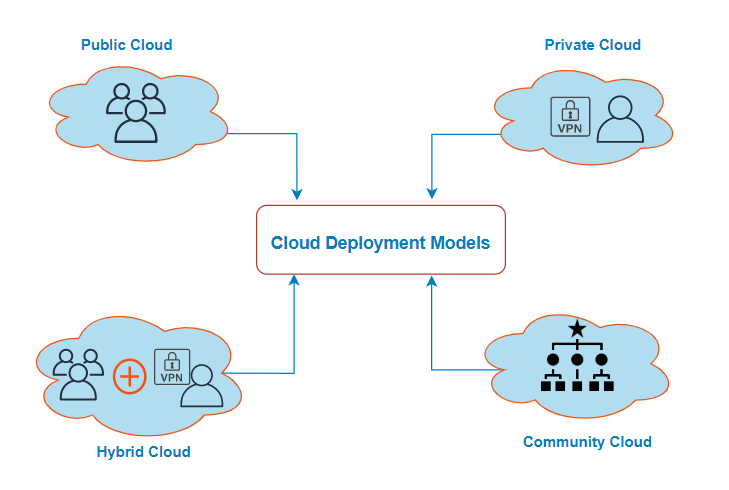
\includegraphics[width=0.5\columnwidth]{{../images/chapter2/cloud3.png}}
					\centering
					\caption{Cloud Deployment Types.}
					\label{fig:cloud3}
				\end{figure}
			
			\subsection{Fog Computing \cite{fogref}}
			\subsubsection{What is Fog Computing}
			Fog computing or fogging is a term coined by CISCO company, it is a decentralized computing infrastructure in which data, compute, storage, and applications are located somewhere between the data source and the cloud. Fog computing brings the advantages and power of the cloud closer to where data is created and acted upon with the aim of solving the problems faced by cloud computing during IoT data processing. 
			
			\subsubsection{Fog Architecture}
			As shown in Fig. \ref{fig:fog1} \textbf{Fog architecture consists of three tiers:}
			\begin{figure}[H]
				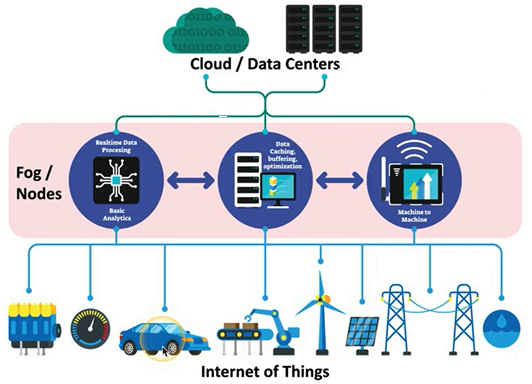
\includegraphics[width=0.5\columnwidth]{{../images/chapter2/fog1.png}}
				\centering
				\caption{Fog Architecture \cite{fogref}.}
				\label{fig:fog1}
			\end{figure}
			\begin{enumerate}
				\item \textbf{Tier 1 – Terminal Layer:} \\
				The terminal layer is the basic layer in fog architecture, this layer includes devices like mobile phones, sensors, smart vehicles, readers, smartcards, etc. The devices which can sense, and capture data are present in this layer. Devices are distributed across several locations separated far apart from each other. The devices in this layer have the property of working in a heterogeneous environment, with other devices from separate technologies and separate modes of communication. 
				\item \textbf{2-Tier 2 – Fog Layer:} \\
				Fog layer includes devices like routers, gateways, access points, base stations, specific fog servers, etc., called as Fog nodes. Fog nodes are located at the edge of a network. An edge can be a hop distance from the end device. They are situated in-between end devices and cloud data centers. Fog nodes are located at the edge of a network. An edge can be a hop distance from the end device. The Fog nodes are situated in-between end devices and cloud data centers. \\
				Fog nodes can be static, e.g., located in a bus terminal or coffee shop, or they can be moving, e.g., fitted inside in a moving vehicle. They provide services to the end devices, and they can compute, transfer and store the data temporarily. Connections between fog nodes and cloud data center are enabled by the IP core networks, providing interaction and cooperation with the cloud for enhancing processing and storage capabilities. 
				\item \textbf{2-Tier 3 – Cloud Layer:} \\
				This layer consists of devices that can provide large storage and machines (servers) with high performance that perform computation analysis and stores data permanently, for back-up and permanent access to the users. The cloud layer lies at the extreme end of the overall fog architecture. It acts as a back-up as well as provides permanent storage for data in a fog architecture. Usually, data that isn’t required at the user proximity is stored in a cloud layer.
			\end{enumerate}
			
			\subsubsection{Why Fog Computing?}
			Cloud computing has three main problems which are \textbf{volume}, \textbf{latency}, and \textbf{bandwidth}. See Fig. \ref{fig:fog2}  
			\begin{itemize}
				\let\labelitemi\labelitemii
				\item \textbf{Volume problem:} occurs due to the terabyte of data produced by billions of devices every day and the continuous increasing of device density, so the current cloud model is unable to process and store this huge amount of data and data need to be filtered. 
				\begin{figure}[H]
					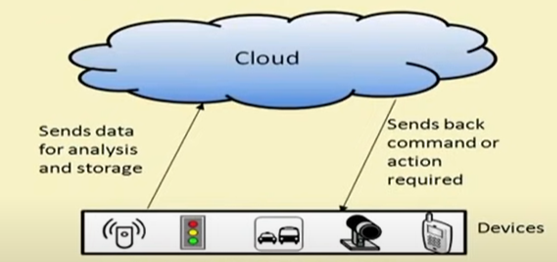
\includegraphics[width=0.5\columnwidth]{{../images/chapter2/fog2.png}}
					\centering
					\caption[]{}
					\label{fig:fog2}
				\end{figure}
				\item \textbf{Latency:} is the time taken by a data packet for a round trip which is an important aspect for handling a time sensitive data. If edge devices send time sensitive data to cloud for analysis and wait for the cloud to give proper action, then it can lead to many unwanted results because while handling time sensitive data, a millisecond can make a huge difference and it the right action reaches the edge devices late this may lead to a disaster or an accident. To solve this problem, Fog divides data into three types based on sensitivity which are time-sensitive data, less time-sensitive data, non-time sensitive data. See Fig. \ref{fig:fog3} 
				\begin{figure}[H]
					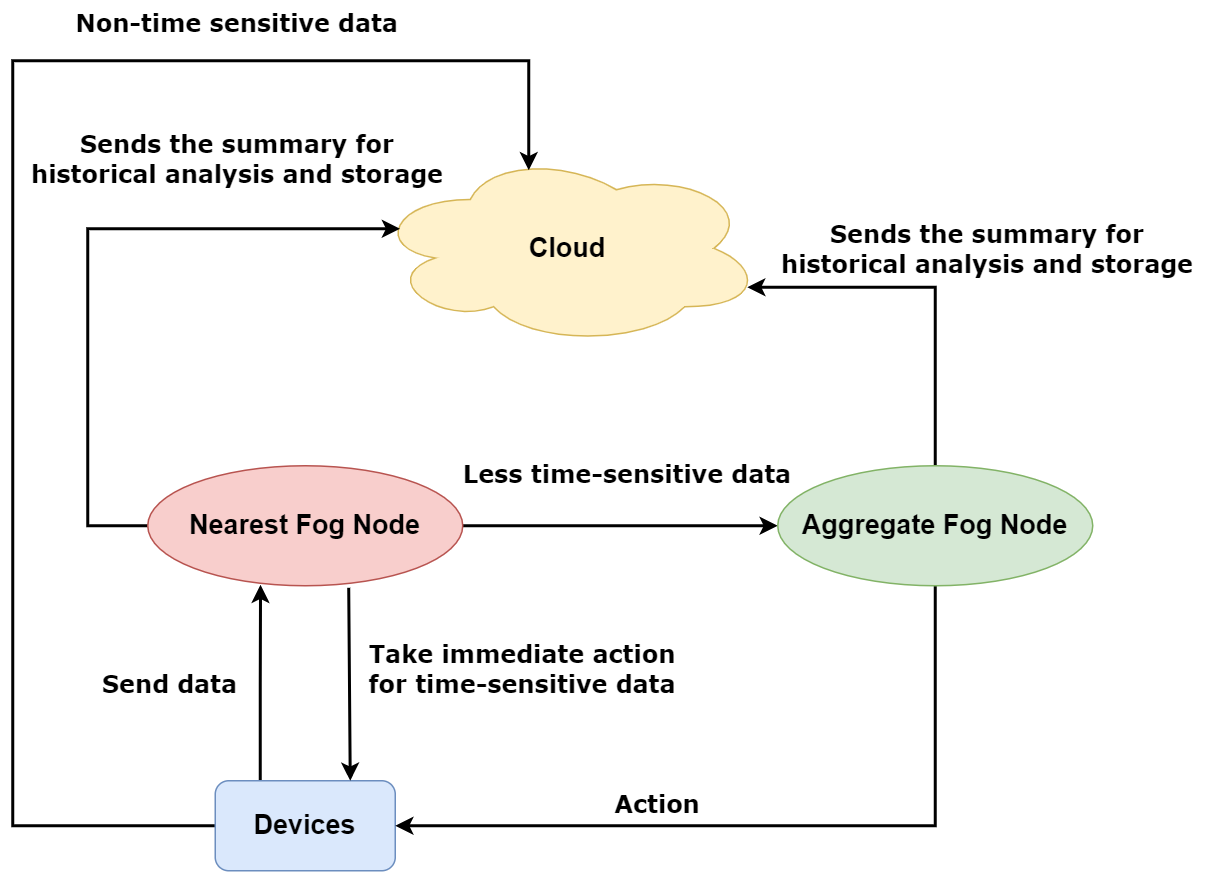
\includegraphics[width=0.7\columnwidth]{{../images/chapter2/fog3.png}}
					\centering
					\caption[]{}
					\label{fig:fog3}
				\end{figure}
				Data is sent form devices to the nearest fog node to be analyzed, if this data is time-sensitive than this fog node sends the immediate action to be taken by the device then sends the summary for historical analysis and storage to the cloud. If data is less-time sensitive, then the nearest fog node redirects this data to an aggregate fog node to determine the appropriate action for this data then sends it back to the devices then sends also sends the summary for historical analysis and storage toe the cloud. non-time sensitive data are sent directly from the devices to the cloud to be analyzed. 
				\item \textbf{Bandwidth:} is defined as the bit-rate of data during transmission. If all the data generated by the IoT devices are sent to cloud for storage and analysis, then, the traffic generated by these devices will be simply gigantic. Handling this kind of traffic will be simply a very hard task. Fog computing solves this problem through distributing the data on different nodes that are placed in the layer between the terminal layer and the cloud layer. 
			\end{itemize}
			
			\newpage
			\subsection{Hardware Components}
			\subsubsection{On-Board Unit (OBU)}
			\begin{figure}[h!]
				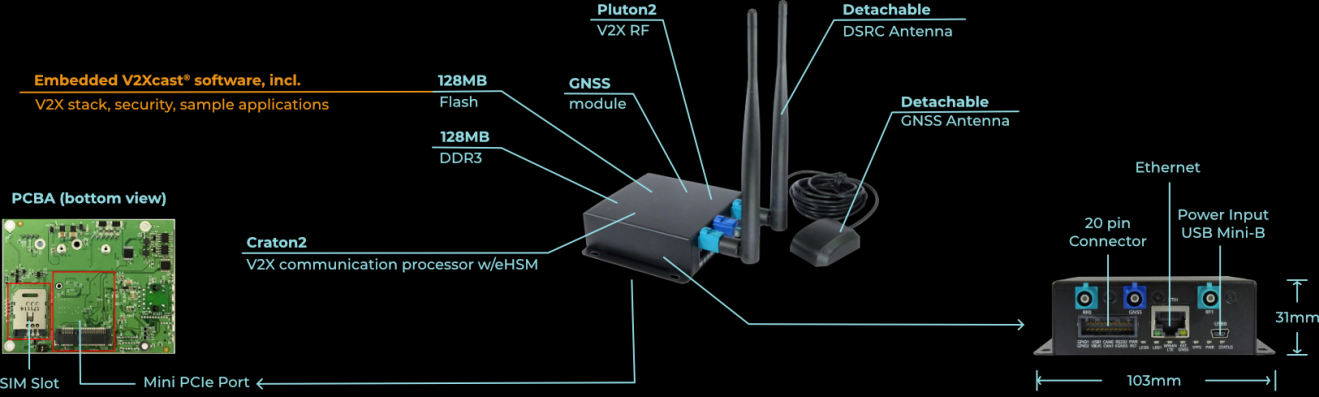
\includegraphics[width=\columnwidth]{{../images/chapter2/obu1.png}}
				\centering
				\caption{An Example of OBU \cite{oburef}.}
				\label{fig:obu1}
			\end{figure}
			OBU stands for On Board Unit. It is an on-board device installed in each vehicle in order to communicate with other OBUs or RSUs. It communicates with other OBU’s or RSU wirelessly through communication protocols such as IEEE 802.11p protocol \cite{singh2020computational}.	
			In Fig. \ref{fig:obu1}, There is an example of a product: \textbf{(Unix 301-U) which works in (-40C to 85C)} \\
			\textbf{As shown in figure, each OBU must have:} 
			\begin{itemize}
				\let\labelitemi\labelitemii
				\item A \textbf{transceiver} consisting of a radio frequency antenna (to access the wireless channel in order to communicate with other OBUs and RSUs) attached to a processor, much like a router. It also has read/write memory to store and retrieve information, and a user interface (to exchange information with the end user, or a connection with a device that has a user interface). 
				\item It also needs to have: a mechanism to generate safety messages to be shared with other OBUs and RSUs (these messages can come directly from user or from automatic processing of sensory data), and the communication module of the device should support: IEEE 802.11p, IEEE1609.1-4 protocols \cite{saini2015close}. 
			\end{itemize}
			\paragraph{Logical block design:}
			\begin{figure}[H]
				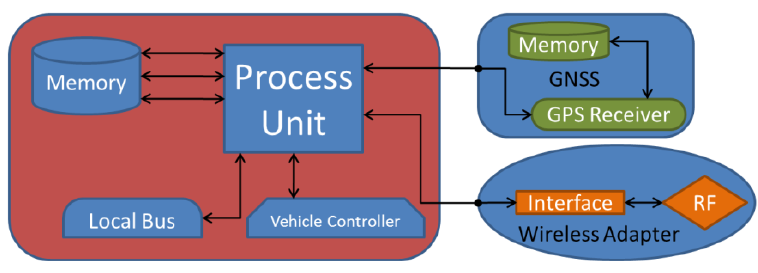
\includegraphics[width=0.7\columnwidth]{{../images/chapter2/obu2.png}}
				\centering
				\caption{Logical Block Design for a fully integrable OBU device \cite{petracca2013board}.}
				\label{fig:obu2}
			\end{figure}
			\textbf{OBU contains three main blocks \cite{petracca2013board}:}
			\begin{itemize}
				\item \textbf{Basic block:} contains process unit, memory, local bus and vehicle controller.
				\item \textbf{GNSS block:} contains memory and GPS receiver.
				\item \textbf{Wireless adapter:} contains interface and RF.
			\end{itemize}
			\paragraph{Why must we have an OBU?} 
			OBU is used to control the congestion in network and to provide reliable and efficient message transfer and data security. It also provides features like ad-hoc networking, wireless communication, geographical routing, etc. \cite{singh2020computational}
			
			\subsubsection{Road-Side Unit (RSU)}
			\begin{figure}[H]
				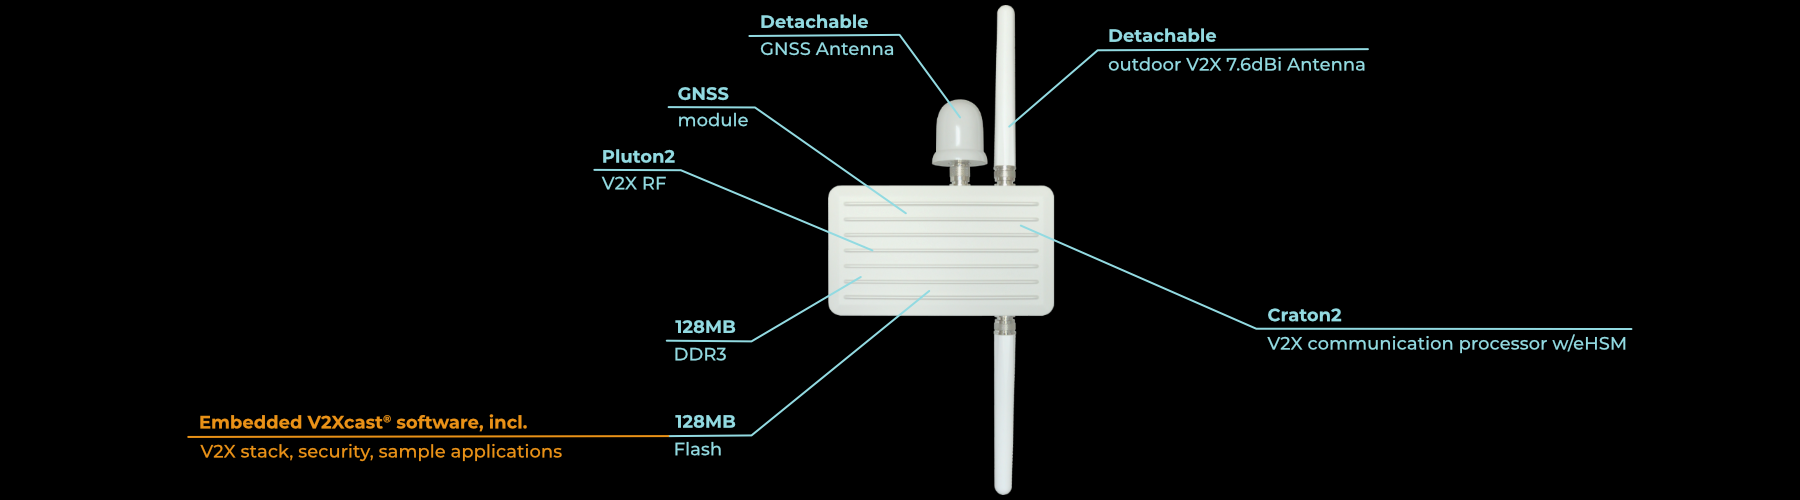
\includegraphics[width=\columnwidth]{{../images/chapter2/rsu1.png}}
				\centering
				\caption{An Example of RSU \cite{rsuref}.}
				\label{fig:rsu1}
			\end{figure}
			RSU stands for Roadside Unit. It is a device which is mostly present at locations like parking area or any roadside area. The RSU uses DSRC (IEEE 802.11p) and broadcasts the message among all vehicles in its coverage area. It acts as a router and provides communication between vehicle and infrastructure. The RSU helps in distributing the messages to different RSU’s or OBU’s, thus extends the network range. It also provides safety information like giving warnings of accident, warning of low bridge, work area, etc. \cite{singh2020computational} \\
			In Fig. \ref{fig:rsu1}, there is an example of a product: \textbf{(Unex 301-U) which works in (-40C to 85C)} \\
			As shown in figure, RSU consists of an antenna, processor, and read/write memory. RSUs have both wired and wireless interfaces. 
			\begin{itemize}
				\let\labelitemi\labelitemii
				\item \textbf{The wireless interface:} is used to communicate with OBUs mounted on vehicles. 
				\item \textbf{The wired interface:} is used to connect with other RSUs and Internet. 
			\end{itemize}
			\paragraph{Main Functionalities of RSU:} 
			\begin{enumerate}
				\item Radio frequency, high power, and long-range antenna to access a wireless medium.
				\item A network stack to run VANET (DSRC) specific network, link, and physical layer protocols.
				\item Forwarding data packets to OBUs in its range and other RSUs.
				\item Aggregation of safety information from OBUs through safety applications.
				\item Working as a gateway to provide Internet connectivity to OBUs.
			\end{enumerate}
			As shown, OBU and RSU are working on WAVE/DSRC \cite{bouk2015hybrid} communication’s layered architecture, and each of them communicate through these protocols. In case of V2I, the OBU communicates directly through its one hop to the RSU. In case of V2V, the OBU is communicating through two hops to the RSU and then through OBU. 
			
			\subsection{Computer Network Concepts}
				A computer network can be defined as a group of hosts connected together to accomplish a certain task. The host can be a computer, a network printer, a server, or any other device that can communicate within the network. To keep everything in order, this network has to be governed by one or more protocols. A protocol is a set of rules governing the communication between two or more hosts. There are two models: TCP/IP model and OSI model \cite{alani2014guide}. We will focus on TCP/IP Model$\ldots$ 
				\begin{figure}[H]
					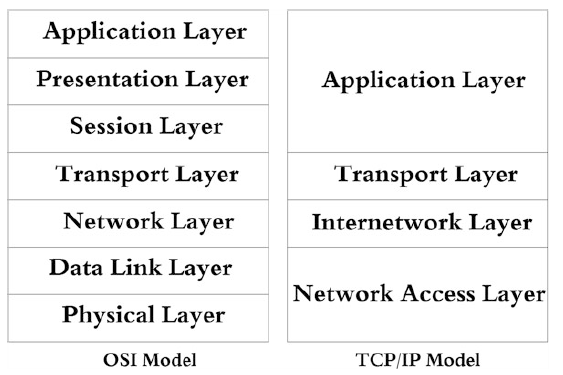
\includegraphics[width=0.6\columnwidth]{{../images/chapter2/network1.png}}
					\centering
					\caption{OSI and TCP/IP reference models: (a) OSI model, (b) TCP/IP model \cite{alani2014guide}.}
					\label{fig:network1}
				\end{figure}
				\subsubsection{TCP/IP Model:}
					TCP/IP model consists of four layers; Network Access layer (or sometimes called Host-to-Network layer), Internetwork layer (sometimes known as Internet layer), Transport layer, and Application layer. The TCP/IP model was created based on a certain set of protocols. Unlike the OSI model which was created as a layered model first with clear defined functions. 
				\subsubsection{TCP/IP model layers:}
					\begin{itemize}
						\let\labelitemi\labelitemii
						\item \textbf{Network Access Layer:}\\
						The TCP/IP standard does not discuss the details of this layer. The duty of this layer is to make sure that the IP packets coming from the Internetwork layer are delivered into a physical link and on the other side, and the opposite is done. Basically, protocols operating in this layer should define the procedures used to interface with the network hardware and access the transmission medium. Mapping the IP addresses used in the Internetwork layer to hardware addresses (such as the MAC address) is yet another duty of this layer.
						\item \textbf{Internetwork Layer:}\\
						Sometimes this layer is called the Internet Layer or the TCP/IP Network Layer. \\
						The main purpose of this layer is to select the best path for the data to travel through from the source to the destination, i.e., routing. The leading protocol operating in this layer is IP. There is a group of supporting protocols that support IP in doing its job, such as the Internet Control Message Protocol (ICMP), Address Resolution Protocol (ARP), and Reverse Address Resolution Protocol (RARP).
						\item \textbf{Transport Layer:}\\
						The transport layer in the TCP/IP model has similar purposes to that of the OSI model. It is designed to give the source and destination the ability to have end-to end conversation. \\
						In the TCP/IP model, there are two defined protocols that can operate in this layer; TCP and UDP. These two protocols provide connection-oriented and connectionless communications. Only TCP protocol provides a way of sequencing, such that even if the data segments arrive in a different sequence of which they were sent in, they can be rearranged.
						\item \textbf{Application Layer:}\\
						The application layer is thought of as the crown of the TCP/IP model. The TCP/IP model does not have session nor presentation layers. The designers thought that they were not that necessary. Thus, the application layer in the TCP/IP model handles data representation, encoding, and dialog control. The main duty of this layer is to take data from the applications and deliver it to the transport layer and collect data from the transport layer and deliver it to the correct applications. \\
						The TCP/IP model contains a huge group of high-level protocols that cover a wide range of applications. The most common is the Hyper Text Transfer Protocol (HTTP).
					\end{itemize}
				
			\subsection{Common Threats (Attacks)}
				We consider that the communication channel in between system components is public and insecure. An adversary $A$ can listen to, modify, forge, or delete the content of the transmitted messages. Specifically, we consider that the adversary $A$ can perform the following categories of attacks, including, DDoS attacks, replay attacks, man-inthe-middle attacks, identity theft attacks, traffic analysis attacks, and masquerading attacks \cite{paper11}.
				\begin{itemize}
					\let\labelitemi\labelitemii
					\item \textbf{DDoS attacks:} The objective of denial of service (DoS) attacks is to make the authentication service unavailable, by (1) overwhelming the authentication service with an enormous amount of traffic to make it busy, so that it is unable to provide access to legitimate users, or (2) changing a legitimate user’s authentication information to false data. This type of attack mainly uses the limits of bandwidth and transmission power to bring down the IoV system, since most of the major IoV components are exposed outdoors and have poor protection, so it is easy to interfere with, controlled, or destroyed.
					\item \textbf{Replay attacks:} It consists of intercepting data packets between legitimate parties and relaying them to their destination without
					modification. Its objectives in IoV infrastructure are to intercept data packets between IoV nodes and then forward them to their final destination without any alterations to trigger malicious actions or cause an unknown system state.
					\item \textbf{Man-in-the-middle (MITM) attacks:} An adversary $A$ can secretly relay and even alter the communication between two parties by impersonating them, believing that they are communicating directly, but in fact, the entire conversation is under the control of the adversary $A$. In the IoV system, MITM attacks can cause serious damages not only to properties but also to human lives, as adversary $A$ can provide false information that can lead to dangerous situations such as theft or even death.
					\item \textbf{Identity theft attacks:} The adversary $A$ covers up under a false identity by using an alleged authenticity from a legitimately authenticated IoV node, broadcasting false and harmful messages,
					or carrying out malicious attacks.
					\item \textbf{Traffic analysis attacks}: It is based on the perception of the adversary $A$ on the network. In this type of attack, the adversary $A$ does not have to compromise the data. Instead, $A$ simply eavesdrops on network traffic to find vital information such as the location of key nodes, routing patterns, and application behavior patterns.
					\item \textbf{Masquerading attacks:} The adversary $A$ can obtain critical information by pretending to be a legitimate node. In IoV, masquerade attacks can bring deadly threats to the network while attackers can conceal their identities with spoofed objects.
					\item \textbf{Session-key compromise:} If the adversary $A$ can manage to compromise the session key, every piece of encrypted data will be available for him/her. $A$ will be able to read, write, delete and forge messages, terminate the session, and many other malicious actions.
					\item \textbf{51\% attacks:} also known as a majority attack, occurs when a single person or group of people gains control of over 50\% of a blockchain’s hashing power. That is usually achieved by renting mining hash power from a third party. Successful attackers gain the ability to block new transactions from being confirmed as well as change the ordering of new transactions. It also allows the malicious agents to essentially rewrite parts of the blockchain and reverse their own transactions, leading to an issue known as double spending. This problem was traditionally an issue faced mostly by electronic payments where a network was incapable of proving that two or more people didn’t spend the same digital asset. 
					\item \textbf{Sybil attacks:} The Sybil attack is an attack wherein a reputation system is subverted by forging identities in peer-to-peer networks. The lack of identity in such networks enables the bots and malicious entities to simulate fake GPS reports to influence social navigation systems. The Sybil attack is more critical in a disaster situation where people are willing to help the distressed person. The vulnerability could be misused to compromise people's safety. 
				\end{itemize} 
			
			\subsection{Simulation Tools and Frameworks}
				\subsubsection{OMNET++}
				OMNET++ \cite{omnet_sim} is an extensible, modular, component-based C++ simulation library and framework, primarily for building network simulations. “Network” includes wired and wireless communication networks, on-chip networks, queuing networks, etc. Domain-specific functionality such as support for sensor networks, wireless ad-hoc networks, Internet protocols, performance modeling, photonic networks, etc., are provided by model frameworks, developed as independent projects. In OMNET++, there are extensions for real-time simulations, network emulation, database integration, SystemC integration, and several other functions. 
				
				\subsubsection{Veins Framework}
				Veins \cite{sommer2019veins} is a model library for (and a toolbox) OMNeT++, which supports researchers conducting simulations involving communicating road vehicles; either as the main focus of a study (such as Vehicular Ad Hoc Networks - VANETs) or as a component (such as in Intelligent Transportation Systems - ITS). It is an open-source software; It is free to download, adapt, and use. The model library includes a full stack of simulation models for investigating communicating vehicles and infrastructure. \\
				Veins does not include custom mobility models of road vehicles. Rather, it has simulations establish a connection to a dedicated road traffic simulator which is running as a separate process, The road traffic simulator that Veins was designed to interoperate with is Simulation of Urban Mobility (SUMO). SUMO can simulate medium to large road networks of cities, urban areas, highways, and freeways. On those, it can simulate the movement of road vehicles. 
				
				\subsubsection{SUMO Framework}
				Simulation of Urban Mobility (SUMO) \cite{sumo} is an open source, highly portable, microscopic, and continuous road traffic simulation package designed to handle large road networks. It allows for intermodal simulation including pedestrians and comes with a large set of tools for scenario creation. It allows to simulate how a given traffic demand which consists of single vehicle moves through a given road network. The simulation allows to address a large set of traffic management topics. It is purely microscopic as each vehicle is modelled explicitly, has an own route, and moves individually through the network. Simulations are deterministic by default but there are various options for introducing randomness. 
	
				\subsubsection{FogNetSim++ Framework}
				FogNetSim++ \cite{qayyum2018fognetsim++} is a toolkit for modeling and simulation of distributed fog environment. it provides users with detailed configuration options to simulate a large fog network. FogNetSim++ enables researchers to incorporate customized mobility models, fog node scheduling algorithms, and manage handover mechanisms. Through FogNetSim++, a user can simulate heterogeneous devices with varying features. It also supports the handover feature to track the source or requested device. Thus, after computation, results can be delivered through different fog nodes deployed at the distinct geographical region. \\
				FogNetSim++ provides a facility to create a network environment that allows the static and dynamic nodes in the network and use various fog protocols for communication, such as Message Queue Telemetry Transport (MQTT), Constrained Application Protocol (CoAP), and Advanced Message Queuing Protocol (AMQP). The FogNetSim++ includes a range of mobility models, such as StationaryMobility, StaticGridMobility, CircleMobility, LinearMobility, TractorMobility, RectangleMobility, and TractorMobility. Users can extend these models to fulfill their requirements. All the fog nodes are managed through a central broker, thus various resource scheduling algorithms can also be incorporated in the proposed simulator.
				
				\subsubsection{AVISPA Tool}
				The AVISPA \cite{vigano2006automated} (Automated Validation of Internet Security Protocols and Applications) tool provides a suite of applications for building and analyzing formal models of security protocols. Protocol models are written in the High Level Protocol Specification Language, or HLPSL(High Level Protocols Specification Language). AVISPA provides a language called the High Level Protocol Specification Language (HLPSL) for describing security protocols and specifying their intended security properties, as well as a set of tools to formally validate them.
		
		\newpage
		\section{Related Work}
			\subsection{A lightweight anonymous cross-regional mutual authentication scheme using blockchain technology for internet of vehicles \cite{paper1}}
			In this paper, the authors proposed a scheme (shown in Fig. \ref{fig:paper1-1}) where the Trust Authority (TA) are responsible for Data processing, Integrating, recasting data send by each vehicle and managing the Vehicle Nodes (VN) which are responsible for data acquisition and data communication devices with the Road-Side-Units (RSU) are responsible for data perception and communication build up on the road in addition to data forwarding to the trusted authority, thus forming the Internet of Vehicles (IoV). \\
			For the reason that vehicle nodes on the IoV are known for it’s mobility and there are cross-regional authentication and key agreement the authors propose a decentralized data storage system in the form of blockchain using Proof of Work (PoW) as a consensus mechanism which require high power consumption so the system stability is insured and the failure of the entire network will not occur due to the failure of on trusted authority and the Blockchain would be employed in the cloud server layer of the IoV which will be time consuming as the cloud connection won’t be sufficient for hard real time services. So, Each trust authority in the cloud server layer stores the data related to identification, registration, authentication and key agreement for each vehicle stored in the blockchain to tampered proof. \\
			\begin{figure}[H]
				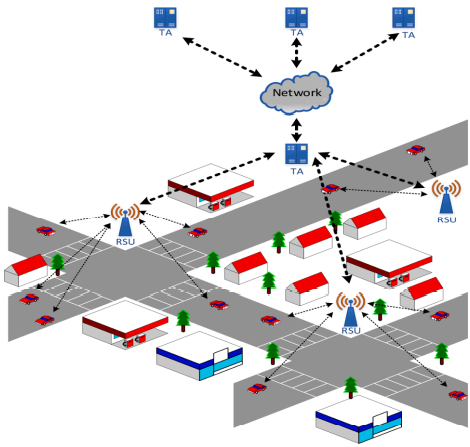
\includegraphics[width=0.55\columnwidth]{{../images/chapter2/paper1-1.png}}
				~
				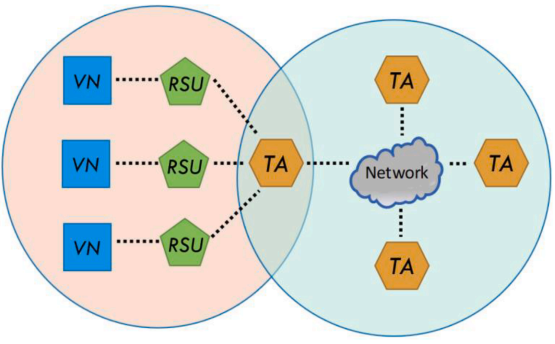
\includegraphics[width=0.4\columnwidth]{{../images/chapter2/paper1-2.png}}
				\centering
				\caption{(a) The architecture of a typical IoV system. (b) The network model for IoV \cite{paper1}.}
				\label{fig:paper1-1}
			\end{figure}
			\subsection{Efficient Distributed Admission and Revocation using Blockchain for Cooperative ITS \cite{paper2}}
			A fully distributed vehicle admission/revocation scheme (architecture shown in Fig. \ref{fig:paper2-1}) that could alleviate the computation overhead and enhance the response time while improving the overall system security is proposed  in, it proposes the use of Blockchain to keep track of the certificate of each vehicle (valid or revoked) in distributed and immutable records rather than the other solutions that depend on Public Key Infrastructure (PKI) which is mainly based on Certificate Authority (CA) that acts as a trusted third party to issue/revoke digital certificates. This PKI-based systems have some problems such as depending mainly on the use of digital certificates for authentication to secure inter-vehicle communication, imposing significant overhead on vehicles since it is computationally demanding and requires validation of the certificate within a limited period and the single point of failure that results from relying on a central node for deciding on issuing and revoking certificates. \\
			The paper solves the single point of failure problem that exits in the PKI-based systems through a blockchain-based system that take the advantage of the distributed nature of the blockchain and the immutability. When a vehicle tries to join to the system it will pass through a set of processes, first Registration, then admission or revocation and misbehavior notification if there a wrong action occurs, and all these processes occur in a completely decentralized manner. \\
			the system support vehicle registration, admission, misbehavior notification and revocation in a completely decentralized manner. Moreover, it eliminates the inherent heavy computation when verifying digital certificates and enables authentication using a simple lookup function. the limitation in this system is that it needs high storage because the number of transactions on the blockchain is proportional to the number of vehicles and revocation/re-registration events, which could be very large. 
			\begin{figure}[H]
				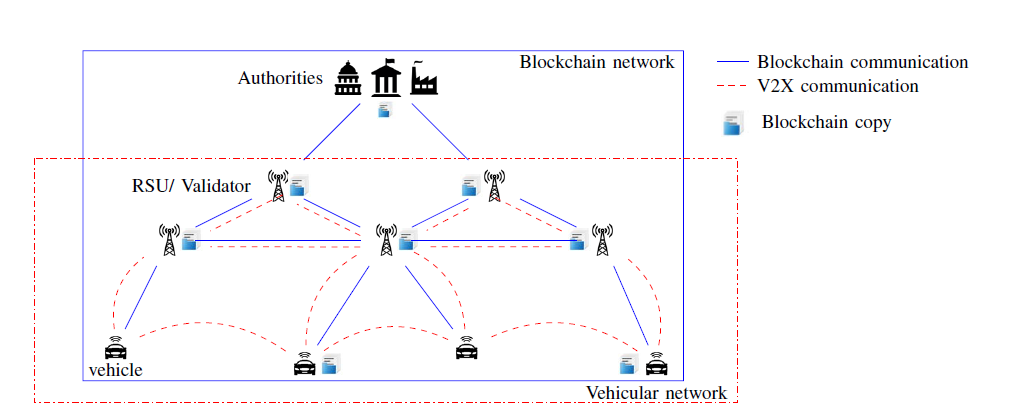
\includegraphics[width=0.8\columnwidth]{{../images/chapter2/paper2-1.png}}
				\centering
				\caption{Architecture of the Proposed Model \cite{paper2}.}
				\label{fig:paper2-1}
			\end{figure}
			\subsection{An Improved Authentication Scheme for Internet of Vehicles Based on Blockchain Technology \cite{paper3}}
			This paper proposed an effective decentralized authentication mechanism for Internet of Vehicles based on the Rayleigh consensus algorithm of blockchain technology. They used blockchain technology combined with the PKI authentication mechanism to solve the identity counterfeiting and identity authentication problem between the vehicles, the servers, and the RSUs in the Internet o Vehicles. This combination also can solve the problem of user account management, which includes the multiple logins of the same account or user. They depend on the encryption feature of the blockchain to encrypt the identity information of the vehicle node and prevent the leakage of user information. The blockchain framework is used to design a new key distribution mechanism. The blockchain ledger technology is used to design a new node joining mechanism, and the blockchain consensus technology is further developed to design a new vehicle identity authentication mechanism.
			\subsection{BlockChain: A Distributed Solution to Automotive Security and Privacy \cite{paper4}}
			This paper proposed a novel automotive security architecture (shown in Fig. \ref{fig:paper4-1}) based on BlockChain (BC) due to its distributed nature. This architecture eliminates the need for a centralized control and the privacy of the users is ensured by using changeable Public Keys (PK) for vehicles while the nodes whose identity should be known, including software providers, vehicle manufacturers and cloud storage share a PK that is certified by a third-party Certification authority (CA). The security of this architecture is largely inherited from the strong security properties of the underlying BC technology. The system replaces the traditional Block chain instantiations that suffer from high (processing and packet) overhead and low scalability and throughput with new Block chain instantiations called Lightweight Scalable Blockchain (LSB) which replaces the demand for solving a computational puzzle with a scheduled block generation process, thus eliminating the significant processing overhead of conventional BCs. LSB clusters the network and only the  Cluster Heads (CHs)  which are the Block Manager (i.e. OBMs) manage the blockchain . An OBM verifies a transaction by validating the signature of the transaction participants with their PK. 
			\begin{figure}[H]
				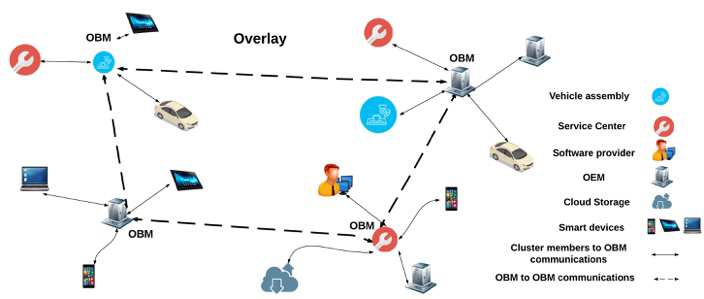
\includegraphics[width=0.9\columnwidth]{{../images/chapter2/paper4-1.png}}
				\centering
				\caption[]{\cite{paper4}}
				\label{fig:paper4-1}
			\end{figure}
			\subsection{Blockchain-Driven Trusted Data Sharing with Privacy-Protection in IoT \cite{paper5}}
			This paper takes the intelligent transportation sensor network as an example and proposes a blockchain-based internet of vehicles (IoV) data secure sharing scheme, called IoVChain (its application is shown in Fig. \ref{fig:paper5-1}), which implements automatic registration, rapid authentication, and reliable sharing method of IoV data through smart contract. In this paper, the secure sharing of IoV data scheme based on blockchain (IoVChain scheme) divides data into public data that can be shared in plain text and private data that must be kept strictly confidential. The model is based on consortium blockchain architecture, which can withstand the risks of some node breakdown and evildoing, and solves the single point of failure problem of the traditional centralized architecture of the IoV. The sensor nodes in the model include Road-Side Unit (RSU) and On-Board Unit (OBU). IoVChain scheme takes the advantage of blockchain, such as tamper-resistance, high security features, to ensure the safety of users' privacy under the condition of the use and sharing of data. Ma Zhaofeng et al. suppose that IoVChain scheme would access data providers including car owners, car manufacturers, 4S stores, car networking companies, insurance companies, and LBS manufactures to integrate the entire process data of vehicles. It would also access more data users, including more auto aftermarket service providers such as e-commerce platforms, auto finance, and government agencies such as traffic management and urban construction, to promote wider data use. IoVChain scheme adopts a data structure based on homomorphic encryption and ZKP, combined with the tamper resistance and open and transparent characteristics of the blockchain. They implemented an IoV data security sharing platform based on Hyperledger Fabric 1.4. For performance evaluation, they used Apache JMeter 4.0 to test the implemented IoVChain platform in an automatic real-time online environment, and evaluate the query efficiency of block according to various conditions, which shows that the proposed solution provides a reliable, safe, efficient and tamper-resistance data security practice for connected vehicles, and it has the potential to be applied in other scenarios of IoT sensor network.
			\begin{figure}[H]
				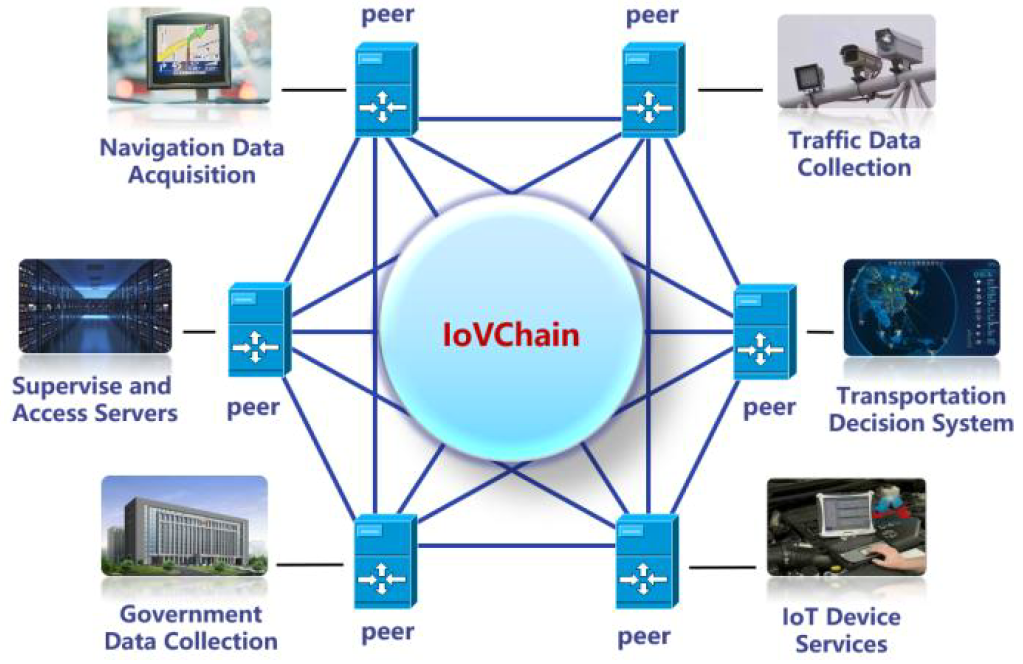
\includegraphics[width=0.7\columnwidth]{{../images/chapter2/paper5-1.png}}
				\centering
				\caption{The application of proposed IoVChain scheme \cite{paper5}.}
				\label{fig:paper5-1}
			\end{figure}
			\subsection{Blockchain-based Internet of Vehicles: Distributed Network Architecture and Performance Analysis \cite{paper6}}
			Tigang Jiang et al. presented a model of the outward transmission of vehicle blockchain data, and give detail theoretical analysis and numerical results, discussed the connections between blockchain and IoV as well as the technical difficulties of implementing blockchain for IoV applications, and conducted theoretical modeling and performance analysis of vehicle networking systems. The objective of the solution is to provide a distributed and secure storage of big data. This paper focuses on the framework and network architecture of the IoV and blockchain including communication performance modeling and analysis method. However, the proposed model does not consider the traffic among vehicles, and the channel reliability of the cellular networks.
			\subsection{A Scalable Protocol for Driving Trust Management in Internet of Vehicles with Blockchain \cite{paper7}}
			\begin{figure}[H]
				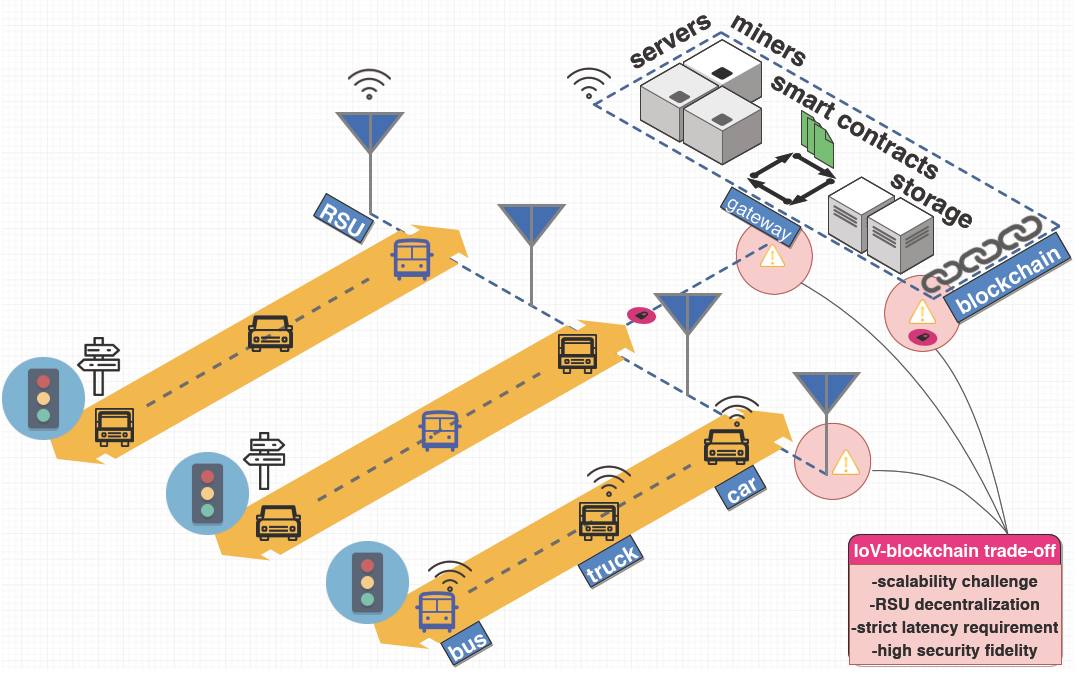
\includegraphics[width=0.8\columnwidth]{{../images/chapter2/paper7-1.png}}
				\centering
				\caption{IoV-blockchain model with the four-way trade-off \cite{paper7}.}
				\label{fig:paper7-1}
			\end{figure}
			Uzair Javaid et al. propose a blockchain-based protocol for IoV using smart contracts, Physical Unclonable Functions (PUF), certificates, and a proof of work (PoW) consensus algorithm. The blockchain and smart contracts provide a secure way of managing vehicle registrations. Physical Unclonable Functions (PUFs) are used to assign a unique identity to each vehicle. Certificates, issued to vehicles by road-side units (RSUs), preserve vehicles' privacy. Moreover, dynamic proof of work (dPoW) consensus algorithm, a type of proof of work, allows the protocol to scale according to the incoming traffic generated by the vehicles. This paper focuses on designing a decentralized trust management protocol for IoV while addressing the four-way trade-off. The four-way trade-off (shown in Fig. \ref{fig:paper7-1}) of blockchain involves these four quintessential factors: \textbf{Scalability}, the quantative measure of of the ability of a blockchain to handle and process transactions such that a blockchain should be able to handle high volumes of transactions supported by a wide range of applications. \textbf{Decentralization}, the distribution of control or resources in a blockchain which allows it to achieve different objectives such as single point of failure. \textbf{Latency}, the time taken for a transaction to be verified or confirmed and added to a block in a blockchain, and become irreversible. \textbf{Security}, the guarantee for the immutability of a ledger in a blockchain and the data it contains, which is known by its robustness and resistance to attacks such as 51\%, Sybil, and DDoS. In this paper, they also present a formal security analysis of the proposed model. The performance evaluation and efficiency in terms of the four-way trade-off of blockchain show that they could outperform many of state-of-the-art existing protocols in many aspects. They also present a case study along with a comparative analysis, which confirms that their protocol can provide superior decentralized trust management for IoV. 
			\newpage
			\subsection{A Blockchain-Based Multi-Factor Authentication Model for a Cloud-Enabled Internet of Vehicles \cite{paper8}}
			This paper is concerning of problem of ineffective authentication techniques which leads to attacks as adversiers can easily exploit the weak authentications, specially, in multi authentication phase. The aim is to harden the authentication through using block chain-based MFA(Multi factor authentication) with using SSO (single sign on) in VC (Vehicular cloud) system, and to certain the confidentiality and integrity of the system. The paper based mainly in Karla and Sood's approach which use an Ecc (Elleptic Curve Cryptography) with eppta (embedded probablestic polynomial time algorithm) to gurantee a higher security to the system, In purposed solution, in blockchain environment the generated Hsh(Hash) will be three times stronger: (New Ds*Ds+Proof-of-work(PoW)+ Hash) which make the adversary need to compute quadrillions of computations to generate the blockchain hash when he tries to eavesdrop, conduct a brute force, or change the immutability of the blockchain. Although the system has very strong authentication, it has a very remarkable problem which are: Reliability and Complexity. The problem of Reliability and Complexity is came from a many overlapping steps in generating the Ds (Digital Signature) and modified Hash, which makes a problem of power consumption and then applying them in environment of Cloud system with SSO which make it also sometimes not applicable in any environments, but environment of 5G and smart cities. 
			\subsection{Enhanced IoV Security Network by Using Blockchain Governance Game \cite{paper9}}
			\begin{figure}[H]
				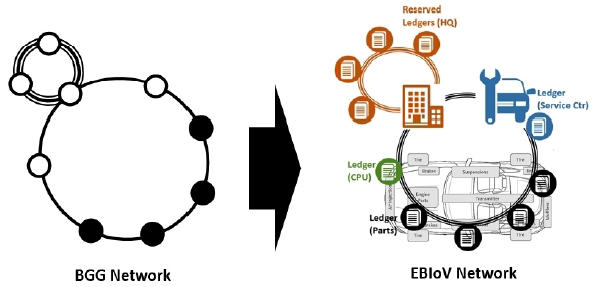
\includegraphics[width=0.9\columnwidth]{{../images/chapter2/paper9-1.png}}
				\centering
				\caption{Adapting BGG for the EBIoV architecture \cite{paper9}.}
				\label{fig:paper9-1}
			\end{figure}
			In this paper, The system is deals with a Blockchain Governance Game (BGG) (shown in Fig. \ref{fig:paper9-1}), which is a system model of a The BGG is a mathematically proven game model to develop optimal defense strategies to protect systems from attackers and find best strategies towards preparation of preventing a network malfunction, the system applies BGG in connected vehicles in the IOV system. Here, the attacker is not an adversary out of the system, but he is one of the miners of the system. The problem of 51\% attack. So, the system consists of one attacker (the miner which intends to fork a private chain) and one defender (the miner which honestly mines on the public chain) and the aim is to predict the moment for safety operations and to deliver the optimal combination of the number of reserved nodes with the acceptance probability of backup nodes to protect a connected car, these nodes are reserved in cloud by headquarter to support the system before just a while before attack happened. The paper gives us a practical case which demonstrates a network could be implemented for connected car securities, The problem of this approach is: Complexity, as this approach is using a very complex mathematically calculations which leads to a time complexity.
			\subsection{Implementing blockchain technology in the Internet of Vehicle (IoV) \cite{paper10}}
			\begin{figure}[H]
				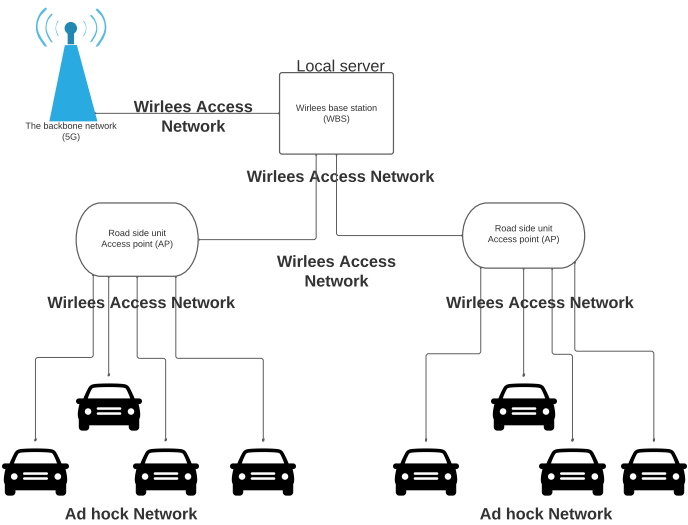
\includegraphics[width=0.7\columnwidth]{{../images/chapter2/paper10-1.png}}
				\centering
				\caption{Network Architecture of the proposed model \cite{paper10}.}
				\label{fig:paper10-1}
			\end{figure}
			This paper aims to utilize a block chain technology to ensure authentic vehicle identification and data authentication which is transmitted from one vehicle to another. The system (shown in Fig. \ref{fig:paper10-1}) is divided into parts: The backbone network (Which provides the internet connectivity and data requirement of IoV operations via the localized WBS), Wireless Base Station (WBS) (Which stores, and controls detailed vehicle information and generates the public keys for vehicles), and the block chain operated network(Which includes communications such like: V2V, V2I, and I2I governed by WBS). The strength of security in this scheme is defined as each block contains: The generic block hash, previous block hash, timestamp, and transaction records/roots. Every block in the block chain contains based transaction security includes both information security (Which guarantees data authenticity, validity, and confidentiality) and transaction security (Which guarantees authenticity and confidentiality). The problem of this system is the size of the block chains which is very large, single point of failure, and time complexity. 
			\subsection{EASBF: An efficient authentication scheme over blockchain for fog computing-enabled internet of vehicles \cite{paper11}}
			\begin{figure}[H]
				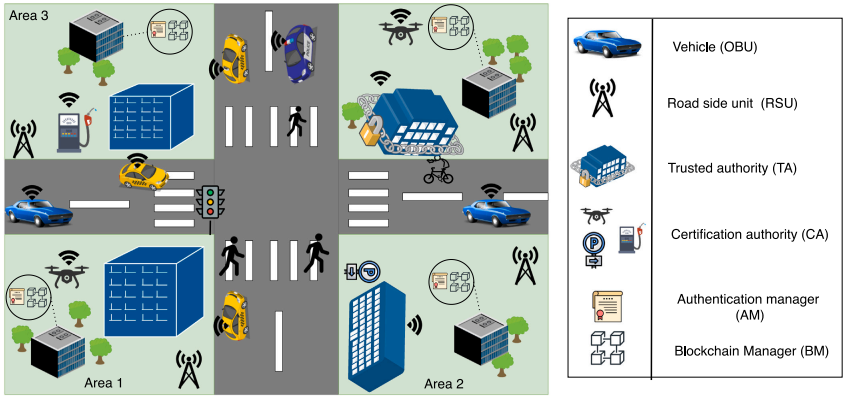
\includegraphics[width=0.8\columnwidth]{{../images/chapter2/paper11-1.png}}
				\centering
				\caption{The Architecture of the proposed scheme \cite{paper11}.}
				\label{fig:paper11-1}
			\end{figure}
			In this paper, the authors propose an authentication scheme using Blockchain deployed using fog computing. The scheme (shown in Fig. \ref{fig:paper11-1}) they propose is formed using many actors starting with Trusted Authority (TA) which is a central secured authority that has the responsibility of registering the OBUs and RSUs nodes. On-Bord-Units (OBU) are the units and sensors installed on vehicles for data collection, acquisition, and communication. Road-Side-Units (RSU) are node in charge of carrying communication for vehicles to communicate with each other and the infrastructure. Blockchain Manager (BM) is responsible for the management of the blockchain and the authentication of the vehicle in a fog area. Certification Authority (CA) is responsible for updating the certification of each vehicle.
			The concept of vehicle Fog Calculation (VFC) has been integrated to improve the efficiency of communication when collecting , organizing, processing, and storing real-time traffic data and minimize latency. The authors propose implementing leading edge cryptography techniques such as one way hash function and elliptic curve cryptography and propose deploying byzantine fault consensus algorithm. But the system has major issue which is the centralized trusted authority which may lead to single point of failure. 
			\subsection{Blockchain Meets VANET: An Architecture for Identity and Location Privacy Protection in VANET \cite{paper12}}
			In this paper, they have mentioned that they divide the privacy protection into three types: location
			privacy protection, trajectory privacy protection and identity privacy protection. For protecting identity and location privacy, they propose UGG, IPP and LPP algorithms with the way of dynamic threshold encryption and k-anonymity unity in the stage of SBMs (all vehicles can receive safety information and be aware of the surrounding traffic environment, such as traffic flow, traffic congestion) upload of blockchain-based VANET. The Idea of k-Anonymity is to protect location of vehicles by combining a set of data with similar attributes to transform sensitive data to low-risk data .To quantify the availability of k-anonymity, they propose two indicators: connectivity and average distance between vehicles . Dynamic threshold encryption is achieved by constructing a polynomial equation which takes the secret S as constant term then dividing the secret into sub-secrets. These sub-secrets are distributed to r different users to keep. any decryption procedure requires judge decision, the decryption key is shared among set of users, cipher text could be decrypted if $r$ users cooperate. 
			\subsection{Hybrid Cryptographic Protocol for Secure Vehicle Data Sharing over Consortium Blockchain \cite{paper13}}
			This paper investigate the potential of the block chain technology in securing and tracking vehicles maintenance and mileage information over a consortium block chain, that is governed by a set of key stakeholders, including an automobile manufacturer, an insurance company, and a service provider. They contributions are many-fold. First, they design a novel architecture to enable the management of vehicles life cycles and data over a decentralized and tamper-proof ledger, hence enabling collaborations and data sharing between the involved parties. For example, vehicles mileages, that are written on the block chain, can enable a vehicle owner to certify the actual value of his car, while it can also enable an insurance company to provide usage-based insurance services (e.g. Pay how/as you drive). Second, they design a novel hybrid cryptographic protocol that address the limitations of existing block chain technologies and enable secure and private data sharing between the involved parties. Vehicles Life-cycle over a Consortium Blockchain have four main steps. Step one: when a consumer acquires a new vehicle; the manufacturer creates a new digital and secure car book on the consortium block chain, and whose access is initially restricted to only the actual car owner and the automotive manufacturer. Step two: Including automatic registration. Step three: maintenance outside dealership network. Step four: resale the car. 
			\subsection{A security scheme based on blockchain and a hybrid cryptosystem to reduce packet loss in IoV \cite{paper14}}
			\begin{figure}[H]
				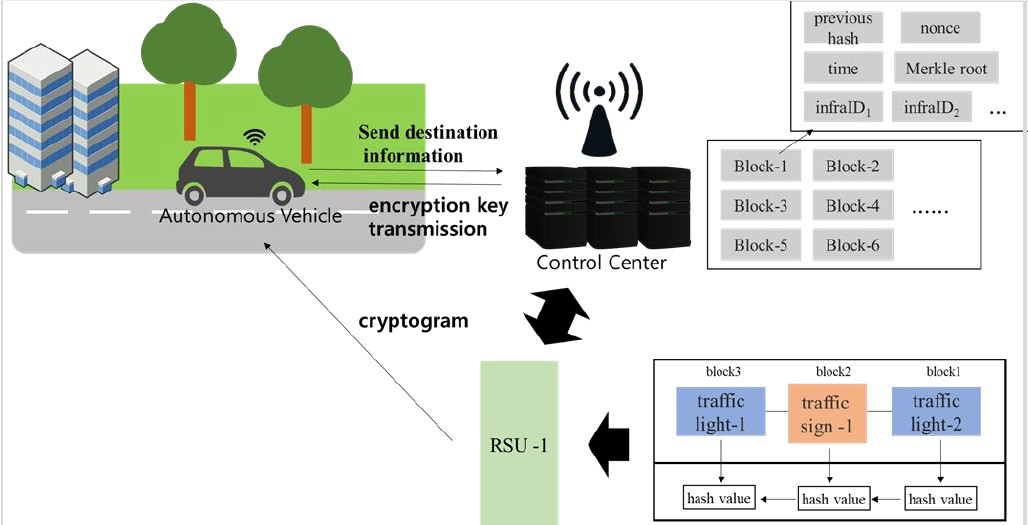
\includegraphics[width=0.75\columnwidth]{{../images/chapter2/paper14-1.png}}
				\centering
				\caption[]{}
				\label{fig:paper14-1}
			\end{figure}
			In this paper, the goal of this scheme (Fig. \ref{fig:paper14-1}) is to reduce the traffic accident caused by packet lose through fast encryption/decryption, In addition, the scalability problem s solved by configuring the blockchain formation only with road infrastructure excluding Roadside Units (RSU). The proposed scheme as follow, The control center verifies the autonomous vehicles and generates a session key for the autonomous vehicle. After that, the control center encrypts the session key with the public key of the autonomous vehicle and transmits it to the corresponding autonomous vehicle. The control center sends a verification request message to the RSU in the path of the autonomous vehicle. The RSU uses information from the infrastructure to form a blockchain. Hash values used to create the blocks utilize information from the road infrastructure communicating with the RSUs. The RSU sends the generated blockchain to the control center, and the control center verifies the blocks. When the block verification is completed, the control center delivers the session key delivered to the autonomous vehicle to the RSU. The control center performs the same verification process for all RSUs in the autonomous vehicle's destination path. 
			\subsection{A secure and computationally efficient authentication and key agreement scheme for Internet of Vehicles \cite{paper15}}
			\begin{figure}[H]
				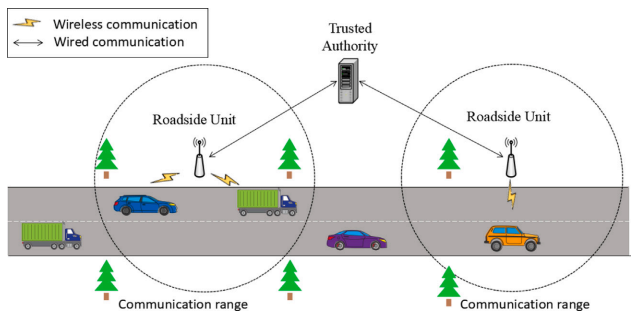
\includegraphics[width=0.75\columnwidth]{{../images/chapter2/paper15-1.png}}
				\centering
				\caption[]{}
				\label{fig:paper15-1}
			\end{figure}
			In this paper, the authors propose a scheme (its architecture is shown in Fig. \ref{fig:paper15-1}) which reduces energy consumption and authentication efficiency, and the actors of the scheme are Trusted Authority (TA) which is responsible for storing information in a trusted cloud server. Road-Side-Units (RSU) are road infrastructure fixed to the roadside which is responsible for authentication vehicles instead of simply acting as intermediate node and communicating with the trusted authority through a wired connection. On-Bord-Units (OBU) are equipped on each vehicle which collect data from surrounding and communicates with the roadside units in a wireless channel via Dedicated Short-Range Communication (DSRC) protocol. \\
			The Authors propose a secure and computationally efficient authentication and key agreement scheme for the IoV using XOR and hash function operations, which mean the scheme uses less energy which is not enough for the security of the system and the cloud server is too slow for the real time services and safety related communication which is a set back in the proposed scheme. 
		
			\begin{sidewaystable}
				\normalsize
				\centering
				\caption{Comparison between Related Schemes.}
				\begin{tabular}{ c  c | c | c | c | c | c | c | c | c |}
					& & \cite{paper1} & \cite{paper2} & \cite{paper3} & \cite{paper4} & \cite{paper5} & \cite{paper6} & \cite{paper7} & \cite{paper8}\\
					\hline
					\multicolumn{2}{|c|}{Blockchain-based} & \ding{51} & \ding{51} & \ding{51} & \ding{51} & \ding{51} & \ding{51} & \ding{51} & \ding{51}\\
					\hline
					\multicolumn{2}{|c|}{Blockchain Type} & Public & Private & \textminus & Private & Consortium & N/A (Private) & Public & Public\\
					\hline
					\multicolumn{2}{|c|}{Decentralization} & \ding{51} & \ding{51} & \ding{53} & \ding{51} & \ding{51} & \ding{51} & \ding{51} & \ding{51}\\
					\hline
					\multicolumn{2}{|c|}{Scalable} & \ding{51} & \ding{53} & \ding{51} & \ding{53} & \ding{53} & \ding{51} & \ding{51} & \ding{51}\\
					\hline
					\multicolumn{2}{|c|}{Use of Certificates} & \ding{51} & \ding{53} & \ding{51} & \ding{51} & \ding{51} & \textminus & \ding{51} & \ding{51}\\
					\hline
					\multicolumn{2}{|c|}{Vehicle Revocation} & \ding{53} & \ding{51} & \textminus & \ding{53} & \ding{51} & \textminus & \ding{51} & \ding{53}\\
					\hline
					\multicolumn{2}{|c|}{Vehicle Registration} & \ding{51} & \ding{51} & \ding{51} & \textminus & \ding{51} & \textminus & \ding{51} & \ding{51}\\
					\hline
					\multicolumn{2}{|c|}{Vehicle Privacy} & \ding{51} & \textminus & \ding{51} & \ding{51} & \ding{51} & \ding{51} & \ding{51} & \ding{51}\\
					\hline
					\multicolumn{2}{|c|}{Unique Vehicle ID} & \ding{51} & \ding{51} & \ding{51} & \ding{51} & \ding{51} & \textminus & \ding{51} & \ding{51}\\
					\hline
					\multicolumn{2}{|c|}{Cryptography Algorithm} & \textminus & \textminus & \textminus & Asymmetric & ZKP & \textminus & ECC with ECDSA & ECC with ePPTA\\
					\hline
					\multicolumn{2}{|c|}{Consensus Algorithm} & PoW & \textminus & Rayleigh & \textminus & PBFT & \textminus & dPoW & \textminus\\
					\hline
					\multicolumn{1}{|c|}{\multirow{6}{*}{Security goals}} & Confidentiality & \ding{51} & \ding{51} & \textminus & \ding{51} & \ding{51} & \textminus & \textminus & \ding{51}\\
					\cline{2-10}
					\multicolumn{1}{|c|}{} & Integrity & \ding{51} & \ding{51} & \textminus & \ding{51} & \textminus & \ding{51} & \ding{51} & \ding{51}\\
					\cline{2-10}
					\multicolumn{1}{|c|}{} & Anonymity & \ding{51} & \textminus & \textminus & \textminus & \ding{51} & \ding{51} & \ding{51} & \ding{51}\\
					\cline{2-10}
					\multicolumn{1}{|c|}{} & Mutual authentication & \ding{51} & \ding{51} & \textminus & \ding{53} & \ding{51} & \textminus & \ding{51} & \ding{51}\\
					\cline{2-10}
					\multicolumn{1}{|c|}{} & Privacy & \ding{51} & \ding{51} & \ding{51} & \ding{51} & \ding{51} & \ding{51} & \ding{51} & \ding{51}\\
					\cline{2-10}
					\multicolumn{1}{|c|}{} & Traceability and Non-repudiation & \ding{51} & \ding{51} & \textminus & \textminus & \ding{51} & \textminus & \ding{51} & \textminus\\
					\hline
					\multicolumn{1}{|c|}{\multirow{8}{*}{Resistance to}} & DDoS attacks & \ding{51} & \ding{51} & \textminus & \ding{51} & \ding{51} & \textminus & \ding{51} & \ding{51}\\
					\cline{2-10}
					\multicolumn{1}{|c|}{} & Replay attacks & \ding{51} & \textminus & \textminus & \textminus & \ding{51} & \textminus & \ding{51} & \ding{51}\\
					\cline{2-10}
					\multicolumn{1}{|c|}{} & Man-in-the-middle attacks & \ding{51} & \textminus & \textminus & \textminus & \ding{51} & \textminus & \textminus & \ding{51}\\
					\cline{2-10}
					\multicolumn{1}{|c|}{} & Identity theft attacks & \ding{51} & \textminus & \textminus & \ding{51} & \ding{51} & \textminus & \ding{51} & \ding{51}\\
					\cline{2-10}
					\multicolumn{1}{|c|}{} & Traffic analysis attacks & \textminus & \textminus & \textminus & \textminus & \textminus & \textminus & \textminus & \ding{51}\\
					\cline{2-10}
					\multicolumn{1}{|c|}{} & Masquerading attacks & \ding{51} & \textminus & \textminus & \textminus & \ding{51} & \textminus & \ding{51} & \ding{51}\\
					\cline{2-10}
					\multicolumn{1}{|c|}{} & Session-key-disclosure attacks & \textminus & \textminus & \textminus & \textminus & \ding{51} & \textminus & \textminus & \ding{51}\\
					\cline{2-10}
					\multicolumn{1}{|c|}{} & 51\% attacks & \ding{53} & \textminus & \textminus & \ding{53} & \ding{51} & \ding{51} & \ding{51} & \textminus\\
					\hline
					\multicolumn{2}{|c|}{RSU-aided authentication function} & \textminus & \ding{51} & \textminus & \ding{53} & \ding{51} & \textminus & \textminus & \ding{53}\\
					\hline
					\multicolumn{2}{|c|}{Vehicle impersonation} & \ding{51} & \textminus & \textminus & \textminus & \textminus & \textminus & \ding{53} & \ding{51}\\
					\hline
					\multicolumn{2}{|c|}{Eliminate single point of failure} & \ding{51} & \ding{51} & \textminus & \ding{51} & \ding{51} & \ding{51} & \ding{51} & \ding{51}\\
					\hline
					\multicolumn{2}{|c|}{Calculate communication overhead} & \ding{51} & \ding{51} & \ding{51} & \ding{53} & \ding{51} & \textminus & \ding{51} & \textminus\\
					\hline
				\end{tabular}
			\end{sidewaystable}
			\begin{sidewaystable}
				\normalsize
				\centering
				\caption{Comparison between Related Schemes (Continued).}
				\begin{tabular}{ c  c | c | c | c | c | c | c | c |}
					& & \cite{paper9} & \cite{paper10} & \cite{paper11} & \cite{paper12} & \cite{paper16} & \cite{paper14} & \cite{paper15}\\
					\hline
					\multicolumn{2}{|c|}{Blockchain-based} & \ding{51} & \ding{51} & \ding{51} & \ding{51} & \ding{51} & \ding{51} & \ding{53}\\
					\hline
					\multicolumn{2}{|c|}{Blockchain Type} & Hybrid & Public & Private & Private & Public & Private (Consortium) & \textminus\\
					\hline
					\multicolumn{2}{|c|}{Decentralization} & \ding{51} & \ding{51} & \ding{51} & \ding{51} & \ding{51} & \ding{51} & \ding{53}\\
					\hline
					\multicolumn{2}{|c|}{Scalable} & \ding{53} & \ding{51} & \ding{51} & \textminus & \textminus & \textminus & \ding{51}\\
					\hline
					\multicolumn{2}{|c|}{Use of Certificates} & \ding{53} & \ding{53} & \ding{51} & \ding{53} & \ding{53} & \ding{53} & \ding{53}\\
					\hline
					\multicolumn{2}{|c|}{Vehicle Revocation} & \ding{53} & \ding{53} & \ding{51} & \ding{53} & \ding{53} & \ding{53} & \ding{51}\\
					\hline
					\multicolumn{2}{|c|}{Vehicle Registration} & \ding{51} & \ding{51} & \ding{51} & \ding{51} & \ding{51} & \ding{51} & \ding{51}\\
					\hline
					\multicolumn{2}{|c|}{Vehicle Privacy} & \ding{51} & \ding{51} & \ding{51} & \ding{51} & \ding{51} & \ding{51} & \ding{51}\\
					\hline
					\multicolumn{2}{|c|}{Unique Vehicle ID} & \textminus & \ding{51} & \ding{51} & \ding{51} & \ding{51} & \ding{51} & \ding{51}\\
					\hline
					\multicolumn{2}{|c|}{Cryptography Algorithm} & \textminus & PKC and SKC & ECC & UGG, LPP and IPP & PK and DSA & Hybrid & \textminus\\
					\hline
					\multicolumn{2}{|c|}{Consensus Algorithm} & No consensus used & \textminus & PBFT & \textminus & \textminus & \textminus & \textminus\\
					\hline
					\multicolumn{1}{|c|}{\multirow{6}{*}{Security goals}} & Confidentiality & \ding{51} & \ding{51} & \ding{51} & \ding{51} & \ding{51} & \ding{51} & \ding{51}\\
					\cline{2-9}
					\multicolumn{1}{|c|}{} & Integrity & \ding{51} & \ding{51} & \ding{51} & \ding{51} & \ding{51} & \ding{51} & \ding{51}\\
					\cline{2-9}
					\multicolumn{1}{|c|}{} & Anonymity & \ding{51} & \ding{51} & \ding{51} & \ding{51} & \ding{51} & \ding{51} & \ding{51}\\
					\cline{2-9}
					\multicolumn{1}{|c|}{} & Mutual authentication & \ding{53} & \ding{53} & \ding{51} & \ding{51} & \ding{51} & \ding{51} & \ding{53}\\
					\cline{2-9}
					\multicolumn{1}{|c|}{} & Privacy & \ding{51} & \ding{51} & \ding{51} & \ding{51} & \ding{51} & \ding{51} & \ding{51}\\
					\cline{2-9}
					\multicolumn{1}{|c|}{} & Traceability and Non-repudiation & \textminus & \textminus & \ding{51} & \textminus & \ding{51} & \textminus & \textminus\\
					\hline
					\multicolumn{1}{|c|}{\multirow{8}{*}{Resistance to}} & DDoS attacks & \textminus & \ding{51} & \ding{51} & \textminus & \textminus & \textminus & \textminus\\
					\cline{2-9}
					\multicolumn{1}{|c|}{} & Replay attacks & \textminus & \ding{51} & \ding{51} & \textminus & \ding{51} & \textminus & \ding{51}\\
					\cline{2-9}
					\multicolumn{1}{|c|}{} & Man-in-the-middle attacks & \textminus & \textminus & \ding{51} & \textminus & \ding{51} & \textminus & \ding{51}\\
					\cline{2-9}
					\multicolumn{1}{|c|}{} & Identity theft attacks & \ding{53} & \ding{53} & \ding{51} & \ding{51} & \ding{51} & \ding{51} & \ding{51}\\
					\cline{2-9}
					\multicolumn{1}{|c|}{} & Traffic analysis attacks & \ding{53} & \ding{51} & \ding{51} & \textminus & \ding{51} & \textminus & \textminus\\
					\cline{2-9}
					\multicolumn{1}{|c|}{} & Masquerading attacks & \ding{51} & \ding{53} & \ding{51} & \textminus & \ding{51} & \textminus & \ding{51}\\
					\cline{2-9}
					\multicolumn{1}{|c|}{} & Session-key-disclosure attacks & \textminus & \textminus & \ding{51} & \textminus & \ding{51} & \ding{51} & \textminus\\
					\cline{2-9}
					\multicolumn{1}{|c|}{} & 51\% attacks & \ding{51} & \textminus & \ding{51} & \textminus & \textminus & \textminus & \textminus\\
					\hline
					\multicolumn{2}{|c|}{RSU-aided authentication function} & \ding{53} & \ding{53} & \textminus & \textminus & \ding{51} & \ding{51} & \ding{51}\\
					\hline
					\multicolumn{2}{|c|}{Vehicle impersonation} & \ding{51} & \ding{53} & \ding{51} & \ding{51} & \ding{51} & \ding{53} & \ding{51}\\
					\hline
					\multicolumn{2}{|c|}{Eliminate single point of failure} & \ding{51} & \ding{53} & \ding{51} & \ding{51} & \ding{51} & \ding{51} & \ding{53}\\
					\hline
					\multicolumn{2}{|c|}{Calculate communication overhead} & \ding{51} & \textminus & \ding{51} & \ding{51} & \ding{51} & \ding{51} & \ding{51}\\
					\hline
				\end{tabular}
			\end{sidewaystable}
		